% ==============================================================================
\chapter{The Timepix3 pixel-beam telescope}
\label{ch:Telescope}
% ==============================================================================  

%% --------------------------------------------- %% 

Testing in a high energy beam is a crucial step in the R\&D for the
pixel detector sensors and readout chips. Test beam data are used at
various stages of the development for evaluating the performance of a
prototype in addition to simulations tools like TCAD and
\textsc{Geant4} simulations.

Pixel-beam telescopes play a key role in the study of position
sensitive sensors with requirements ranging from high radiation
hardness, high resolution and low material budget but also medical
applications amongst others. A telescope is used to reconstruct the
tracks of the particles going through its planes. The track position
is then extrapolated on the Device Under Test (DUT). This allows to
compare the position of the hit on the DUT with the reconstructed
track and extract the position and time resolutions as well as the
efficiency of the device.

For the CLIC vertex detector R\&D, the Timepix3 telescope is used as a
beam reference. This chapter overviews the components of the Timepix3
telescope and its tracking performance. The Timepix3 telescope is
implemented in AllPix simulations (c.f. \cref{sec:AllPix}) and its
performance is compared to the data taken at the CERN SPS. Finally,
the tracking resolution on the DUT is extracted in simulations using
the Monte Carlo Truth position.

%% --------------------------------------------- %%
\section{Experimental setup at the CERN SPS}
\label{sec:CERN_SPS}
The Timepix3 telescope is commissioned and tested at the H6 beam of
the CERN SPS using the $120\,\gev$ pion beam. The assemblies listed in
\cref{tab:Timepix3Assemblies} are tested as DUTs using this
telescope. The beam is configured in such a way to have $\sim2.6
\times 10^6$ particles per spill. The telescope planes are positioned
in a way to give the best tracking resolution for the given beam
energy and the level of multiple scatterings.
%% --------------------------------------------- %%
\section{Components of the Timepix3 telescope}

\subsection{Sensors and mechanics}
The Timepix3 telescope consists of six planes of Timepix3
ASICs~\cite{Timepix3_Poikela} bump bonded to $300\,\micron$ thick
p-in-n planar sensors as shown in \cref{fig:TPX3Telescope}. The planes
are rotated by $9\degrees$ around the x axis (perpendicular to the
beam axis) and the z axis (parallel to the beam axis)
\cite{Akiba:2013yxa}. Given the pixel pitch and the sensor thickness,
this angle mainly leads to clusters of three-hit pixels. Combining the
TOT information, the reconstructed hit position provides sub-pixel
resolution. A tracking resolution of $\sim$$2\,\micron$ on the DUT can
be obtained.


\begin{figure}[htbp]
  \centering
  \begin{tikzpicture}
    \node[anchor=south west,inner sep=0] (image) at
    (0,0){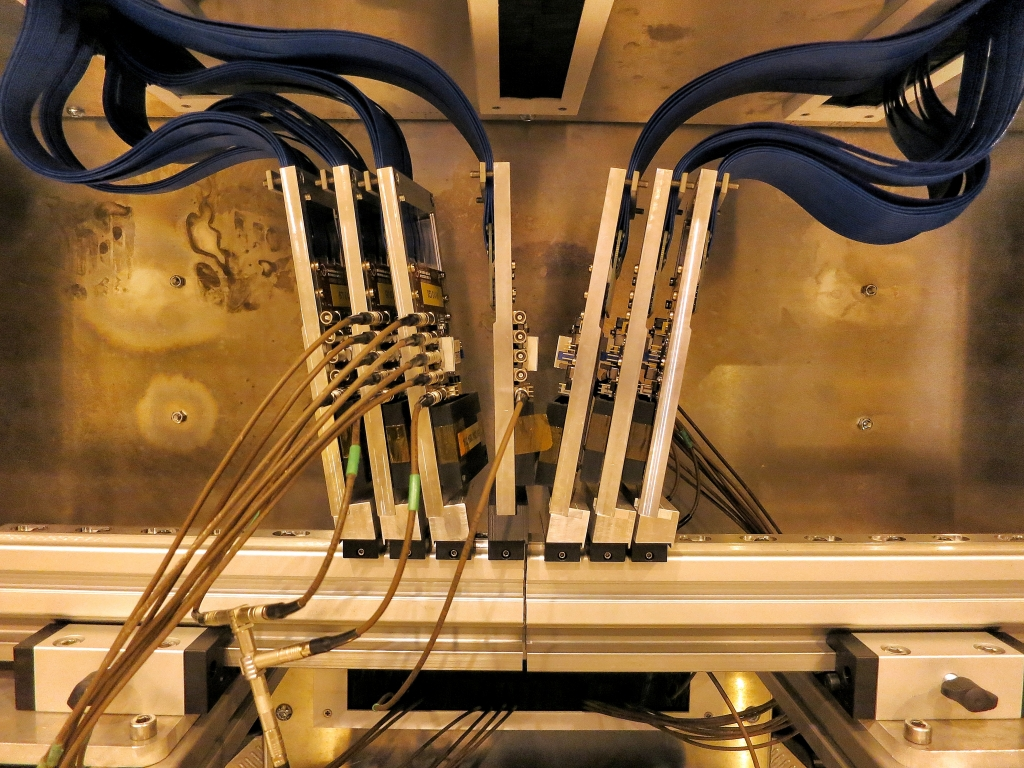
\includegraphics[width=0.6\textwidth]{ActiveEdge/Timepix3Telescope.jpeg}};
    \begin{scope}[x={(image.south east)},y={(image.north west)}]
      \node[above, color=white] at (0.5, 0.85) {Device Under Test};
      \node[above, color=white] at (0.5, 0.78) {(\textbf{DUT})};

      \draw[->, very thick, color=black](0.8, 0.25) -- (0.25, 0.25);
      \node[above, color=black] at (0.5, 0.18) {\textbf{Beam}};
      
      %% \draw[help lines,xstep=.1,ystep=.1] (0, 0) grid (1,1);
      %% \foreach \x in {0,1,...,9} { \node [anchor=north] at (\x/10,0) {0.\x}; }
      %% \foreach \y in {0,1,...,9} { \node [anchor=east] at (0,\y/10) {0.\y}; }
      
    \end{scope}
  \end{tikzpicture} 
  \caption{The Timepix3 beam reference telescope with six planes for
    the tracking and the DUT in the middle inserted perpendicular to
    the beam direction.}
  \label{fig:TPX3Telescope}
\end{figure}

The mechanical support for the telescope planes are optimised in order
to reduce the multiple scatterings of the particles and therefore
improving the tracking resolution. The Timepix3 assemblies are mounted
on a PCB as shown in \cref{fig:Timepix3board_PCB}. An aluminum support
is used to hold the PCB which does not cover the sensor. To protect
the sensors an ABS plastic material is used as cover with a thickness
of 2~mm and placed at a distance of 10~mm away from the PCB (in black
in \cref{fig:TPX3Telescope}). \cref{tab:TPX3TelescopeMaterial}
describes the material (with their thicknesses and radiation lengths)
seen by the particles for each telescope plane which would contribute
to the multiple scatterings. The PCB stacks up eight layers of copper
interlacing with Isola IS410 type material. An average is done to
estimate the total thickness of Copper in the PCB. Behind the PCB a
layer of Copper is used for the cooling of the chip. The total
material budget of a telescope plane is estimated to be
$\sim4\%$~X\textsubscript{0}.

\begin{table}[htbp]
  \centering
  \caption{The material in each telescope plane contributing to the
    multiple scatterings of the particles detected by the sensor where
    X refers to the thickness and X\textsubscript{0} to the radiation
    length (both in millimeters).}
  \label{tab:TPX3TelescopeMaterial}
  \begin{tabular}{l c c c}
    \toprule
    Material & X [mm] & X\textsubscript{0} [mm] & X/X\textsubscript{0} [$\%$] \\
    \midrule
    Cooling material for the chip (Cu) & 0.1 & 14.4 & 0.69 \\
    Isola IS410 in the PCB & 1.475 & 167.6 & 0.88 \\
    Copper in the PCB & 0.125 & 14.4 & 0.87 \\
    ASIC (Si) & 0.7 & 93.7 & 0.75\\
    Sensor (Si) & 0.3 & 93.7 & 0.32\\ 
    Sensor cover (ABS plastic) & 2 & 406.4 & 0.49 \\ \hline
    Total & & & 4 \\
    \bottomrule
  \end{tabular}
\end{table}

\subsection{Coordinates system}
A Cartesian right-handed coordinate system is chosen to describe the
geometry of the telescope. The z-direction is along the beam as shown
in \cref{fig:TPX3Telescope} and the y-direction points vertically in
the up direction.

\subsection{Data acquisition system}
The SPIDR readout system, as described in \cref{sec:TimepixReadout},
is used for the data acquisition of the Timepix3 telescope planes. The
Timepix3 readout ASICs are operated with the data-driven
zero-suppressed readout mode. This system allows to record the data
from all the particles from the SPS spill and generates a large amount
of data for processing offline as described in \cref{sec:recoSoft}.


%% --------------------------------------------- %%
\section{Timepix3 telescope performance}
\label{sec:telescopePerformance}

The Timepix3 telescope is simulated with the \textsc{Geant4}-based
AllPix simulation framework (c.f. \cref{sec:AllPix}). This allows for
a better understanding of the telescope performance, extraction of the
tracking resolution on the DUT and comparison to data. Since AllPix
gives access to the Monte Carlo Truth position (MC position) of the
hits, the true tracking resolution can be obtained by comparing the MC
position with the reconstructed track or hit positions.

\subsection{Timepix3 telescope simulation in AllPix}
In the simulations, the geometry of the telescope is defined as
realistic as possible by taking into account the positions and the
rotations of the telescope planes, the thickness of the sensors and
the pixel pitch. 

The mechanical support for the telescope planes is implemented using
the material as described in
\cref{tab:TPX3TelescopeMaterial}. \textsc{Geant4} provides the class
\textsc{G4Material} which describes the macroscopic properties of the
material used in simulations and contains all the relevant information
on its constituent elements. The density and the radiation length of
the material are the two main properties to be considered for the
simulations. \textsc{Geant4} already provides a material database for
all the standard material such as copper and silicon. For the Isola
IS410, the material G4\_BONE\_COMPACT\_ICRU has the closest radiation
length and density. For the sensor covers in ABS plastic, their
constituent elements
(C\textsubscript{8}H\textsubscript{8}~C\textsubscript{4}H\textsubscript{6}~C\textsubscript{3}H\textsubscript{3}N)
have been implemented as a \textsc{G4Material} in the simulations to
obtain the correct density and radiation length.

\begin{figure}[htbp]
  \centering
  \begin{tikzpicture}
    \node[anchor=south west,inner sep=0] (image) at
    (0,0){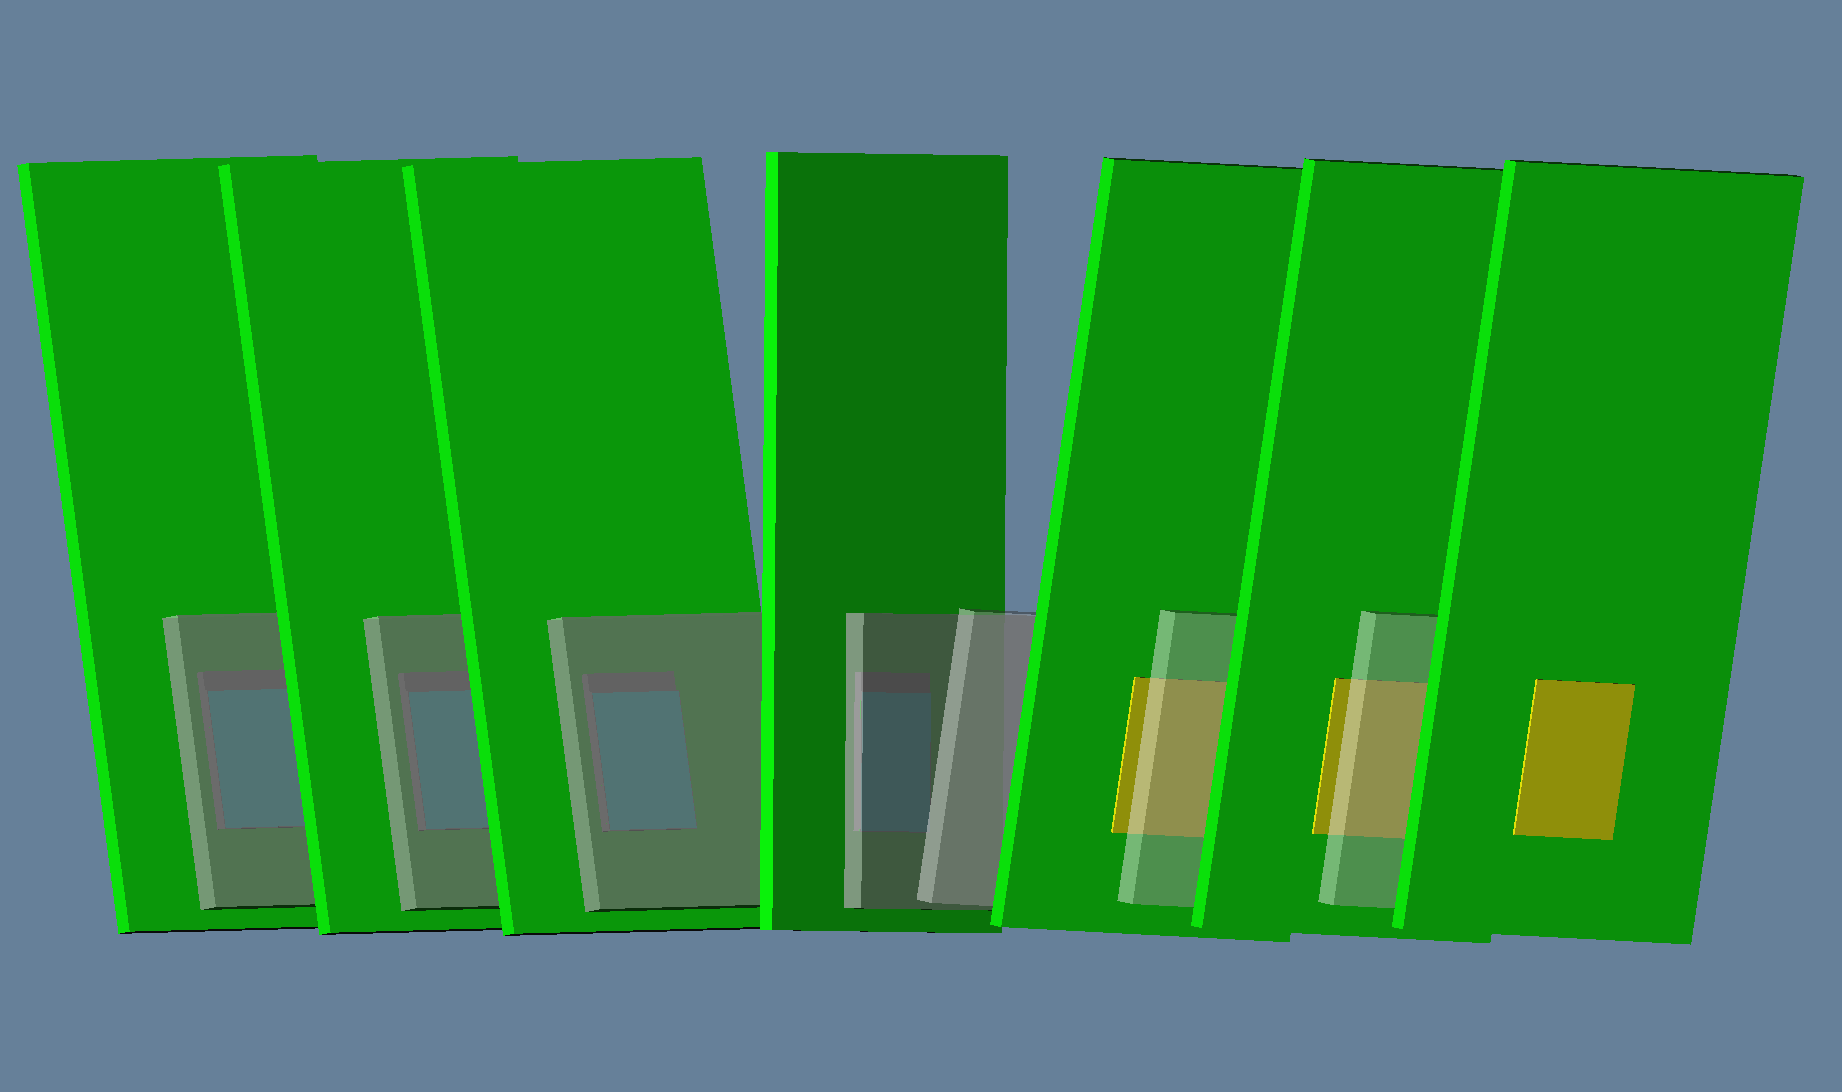
\includegraphics[width=0.6\textwidth]{figures/Telescope/AllpixTelescope.png}};
    \begin{scope}[x={(image.south east)},y={(image.north west)}]
      
      \draw[->, very thick, color=black](0.8, 0.9) -- (0.25, 0.9);
      \node[above, color=black] at (0.5, 0.91) {\textbf{Beam}};
      
      \node[above, color=black] at (0.9, 0.05) {\footnotesize{Plane 0}};
      \node[above, color=black] at (0.75, 0.05) {\footnotesize{Plane 1}};
      \node[above, color=black] at (0.6, 0.05) {\footnotesize{Plane 2}};
      \node[above, color=black] at (0.48, 0.05) {DUT};
      \node[above, color=black] at (0.35, 0.05) {\footnotesize{Plane 3}};
      \node[above, color=black] at (0.2, 0.05) {\footnotesize{Plane 4}};
      \node[above, color=black] at (0.07, 0.05) {\footnotesize{Plane 5}};

      \node[above, color=black] at (0.35, 0.7) {Sensor cover};
      \draw[->, color=black](0.35, 0.7) -- (0.35, 0.45);
      \node[above, color=black] at (0.9, 0.7) {Cooling};
      \draw[->, color=black](0.85, 0.7) -- (0.85, 0.4);

      %% \draw[help lines,xstep=.1,ystep=.1] (0, 0) grid (1,1);
      %% \foreach \x in {0,1,...,9} { \node [anchor=north] at (\x/10,0) {0.\x}; }
      %% \foreach \y in {0,1,...,9} { \node [anchor=east] at (0,\y/10) {0.\y}; }
      
    \end{scope}
  \end{tikzpicture} 
  \caption{The Timepix3 beam reference telescope implemented in AllPix
    with six planes for the tracking and the DUT in the middle
    inserted perpendicular to the beam direction. The sensor covers
    and the chip cooling are shown. The telescope planes numbering
    convention is also shown.}
  \label{fig:Timepix3Telescope_Allpix}
\end{figure}


A digitiser for the Timepix3 readout chips bump-bonded to planar
sensors is defined in AllPix. It simulates the silicon physics by
calculating the diffusion at each \textsc{Geant4} step as described in
\cref{sec:allpix_digitisation}. The contribution of the generated
charge by diffusion in the hit pixel and all its direct neighbouring
pixels is calculated for each step. All the contributions add-up and
finally the charge in each pixel is calculated. Finally a threshold is
applied to each pixel and the electronic noise of the Timepix3 ASIC
also adds up to the charge in each pixel. And finally, the TOT value
is calculated by applying the calibration to each assembly.

\subsection{Single-hit resolution on the telescope planes}

\cref{tab:AllPixTelescopePlanesParams} shows the parameters used for
the simulation of the sensors of the telescope planes. The bias and
the depletion voltages, the sensor type and the threshold values are
the parameters defining the charge sharing and the cluster size
distribution. Therefore they define the intrinsic resolution of the
sensors.

\begin{table}[htbp]
  \centering
  \caption{Parameters used for the simulation of the telescope planes in AllPix.}
  \label{tab:AllPixTelescopePlanesParams}
  \begin{tabular}{cccc}
    \toprule
    Bias voltage [V] & Depletion voltage [V] & Sensor type & Threshold [e-] \\
    \midrule
    50 & 30 & p-in-n & 1000 \\
    \bottomrule
  \end{tabular}
\end{table}


\cref{fig:TelescopeCluSize_data_simu} compares the cluster size
distribution and the charge of the clusters in data and simulations
for the first telescope plane (plane 0).

\begin{figure}[htbp] \centering
  \begin{subfigure}[b]{0.3\textwidth}
    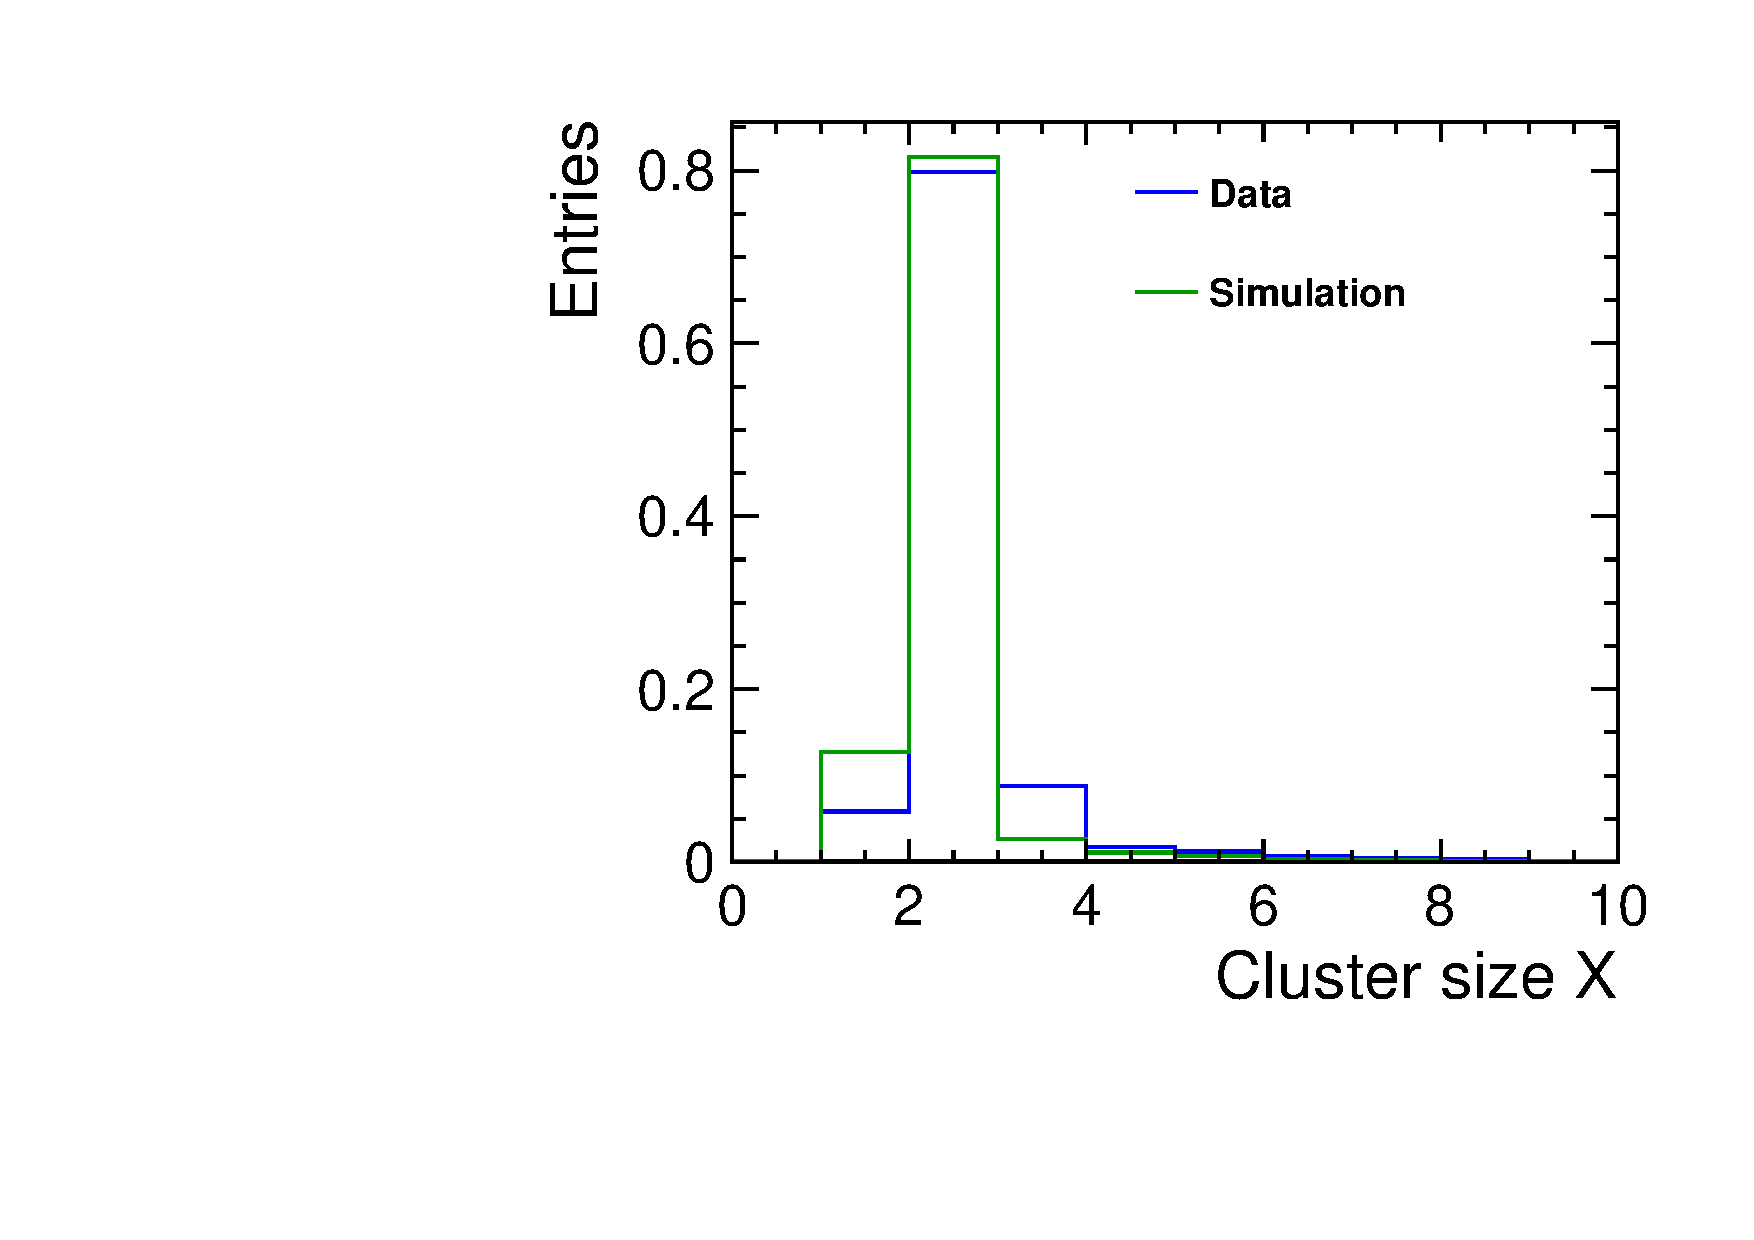
\includegraphics[width=\textwidth]{figures/Telescope/biasedResiduals/clusterSizeX_telescope0_data_simu.pdf}
    \caption{}
  \end{subfigure}\hfill
  \begin{subfigure}[b]{0.3\textwidth}
    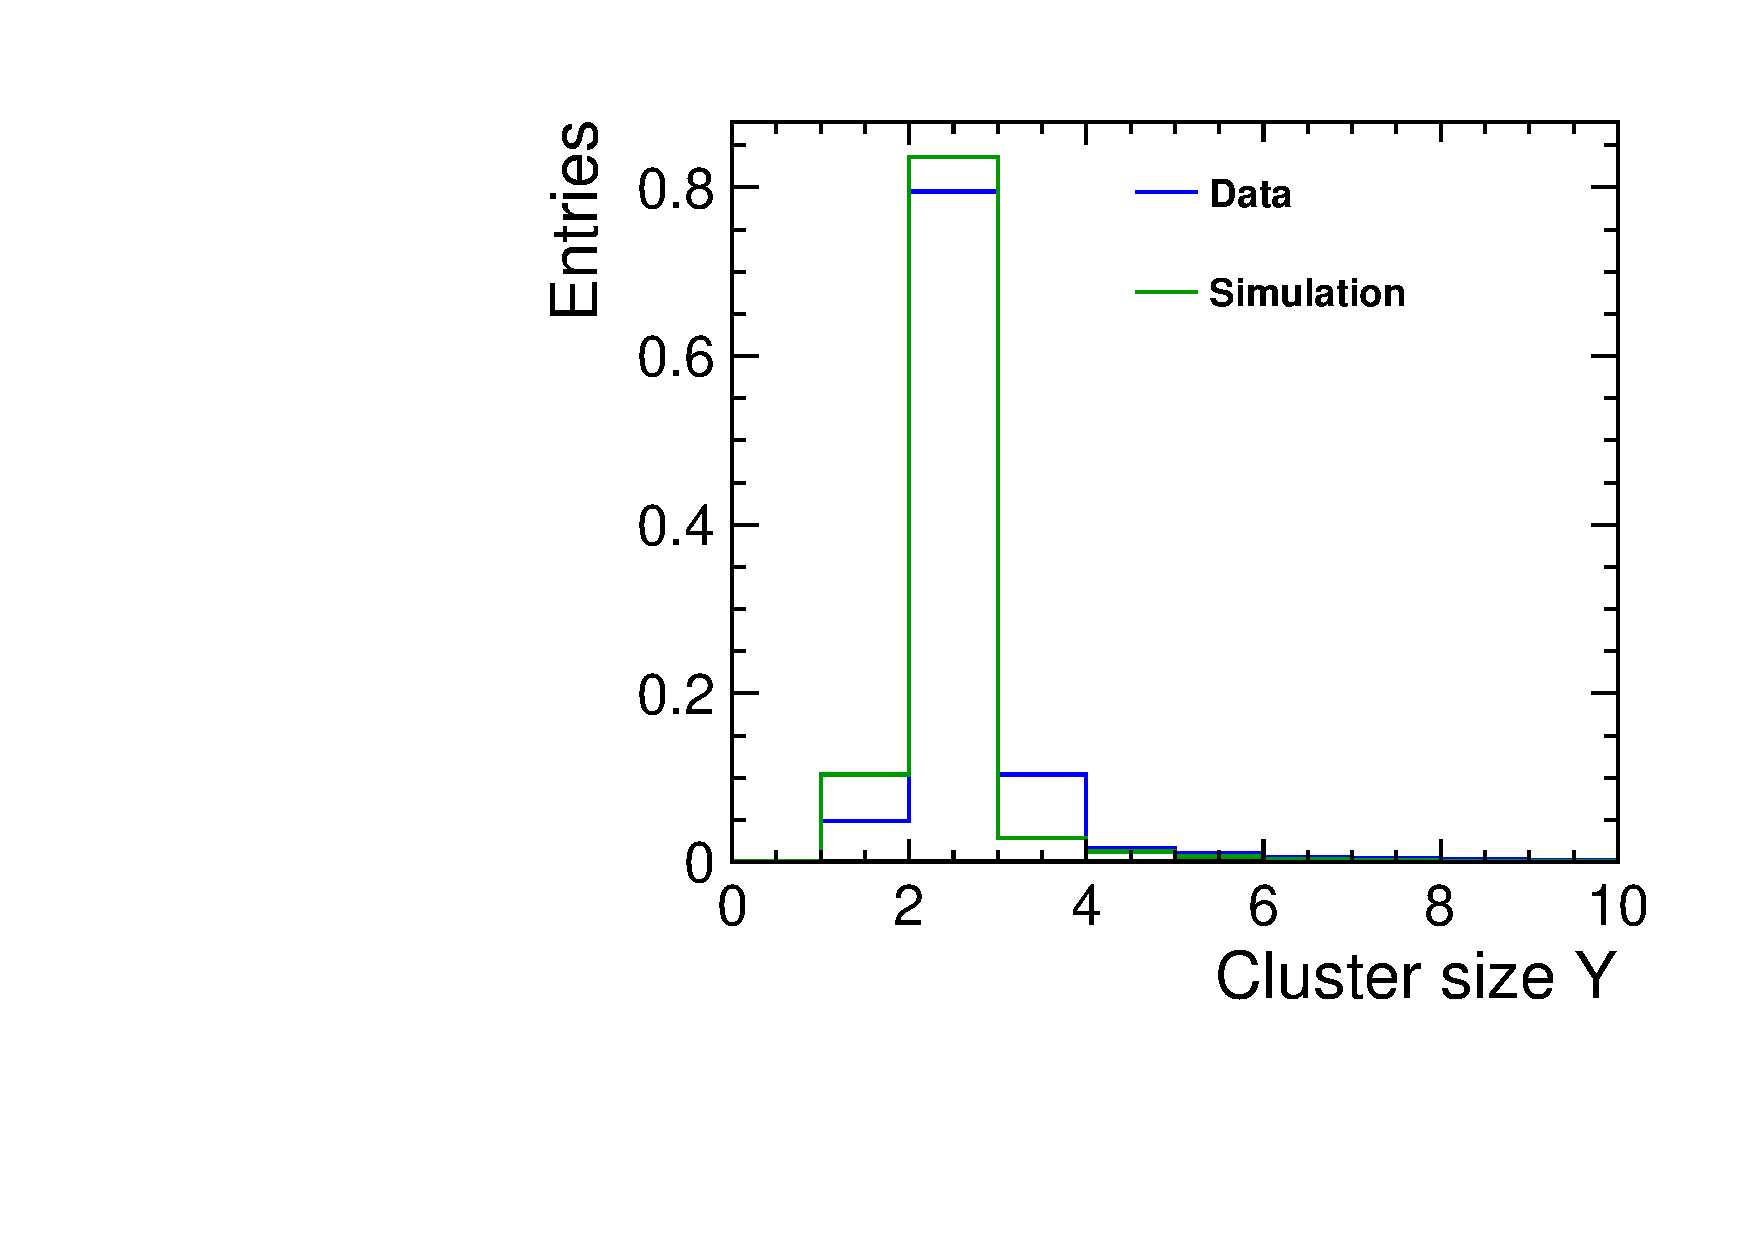
\includegraphics[width=\textwidth]{figures/Telescope/biasedResiduals/clusterSizeY_telescope0_data_simu.pdf}
    \caption{}
  \end{subfigure}\hfill
  \begin{subfigure}[b]{0.3\textwidth}
    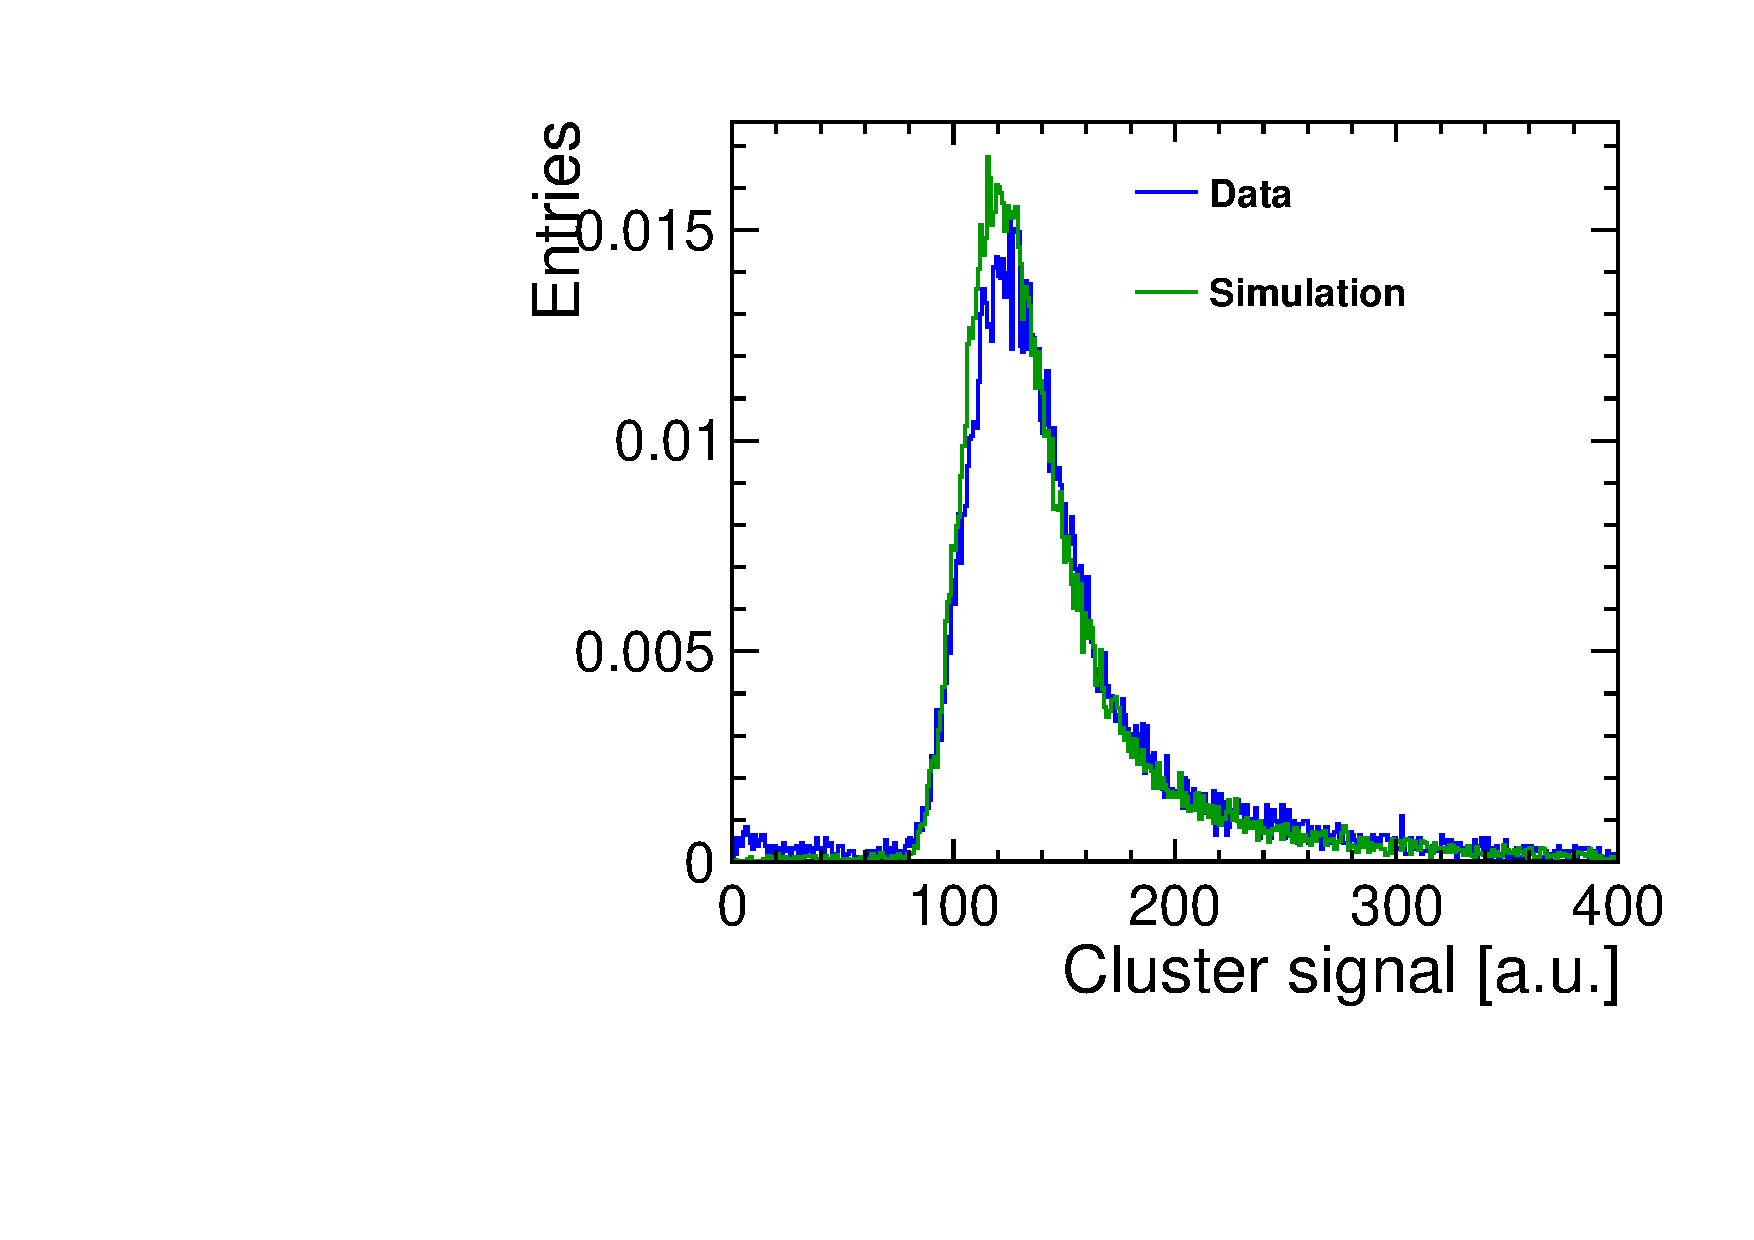
\includegraphics[width=\textwidth]{figures/Telescope/biasedResiduals/clusterSignal_telescope0_data_simu.pdf}
    \caption{}
  \end{subfigure}
  \caption{For the telescope plane 0, the cluster-size distribution in the (a) x direction and (b) y direction. (c) shows the sum of the charge in the cluster in units of TOT.} %data run 661, simulation run 54.
  \label{fig:TelescopeCluSize_data_simu}
\end{figure}

The reconstructed hit on each telescope plane is compared to the Monte
Carlo Truth position (x\textsubscript{MC} and y\textsubscript{MC})
obtained by AllPix simulations. \cref{fig:TelPlane0_MC_hit} compares
the hit resolution on the first telescope plane in x and y
directions. These resolutions are in fact the intrinsic resolution of
the telescope planes sensors and depends on their thickness, charge
sharing and rotations.

\begin{figure}[htbp] \centering
  \begin{subfigure}[b]{0.45\textwidth}
    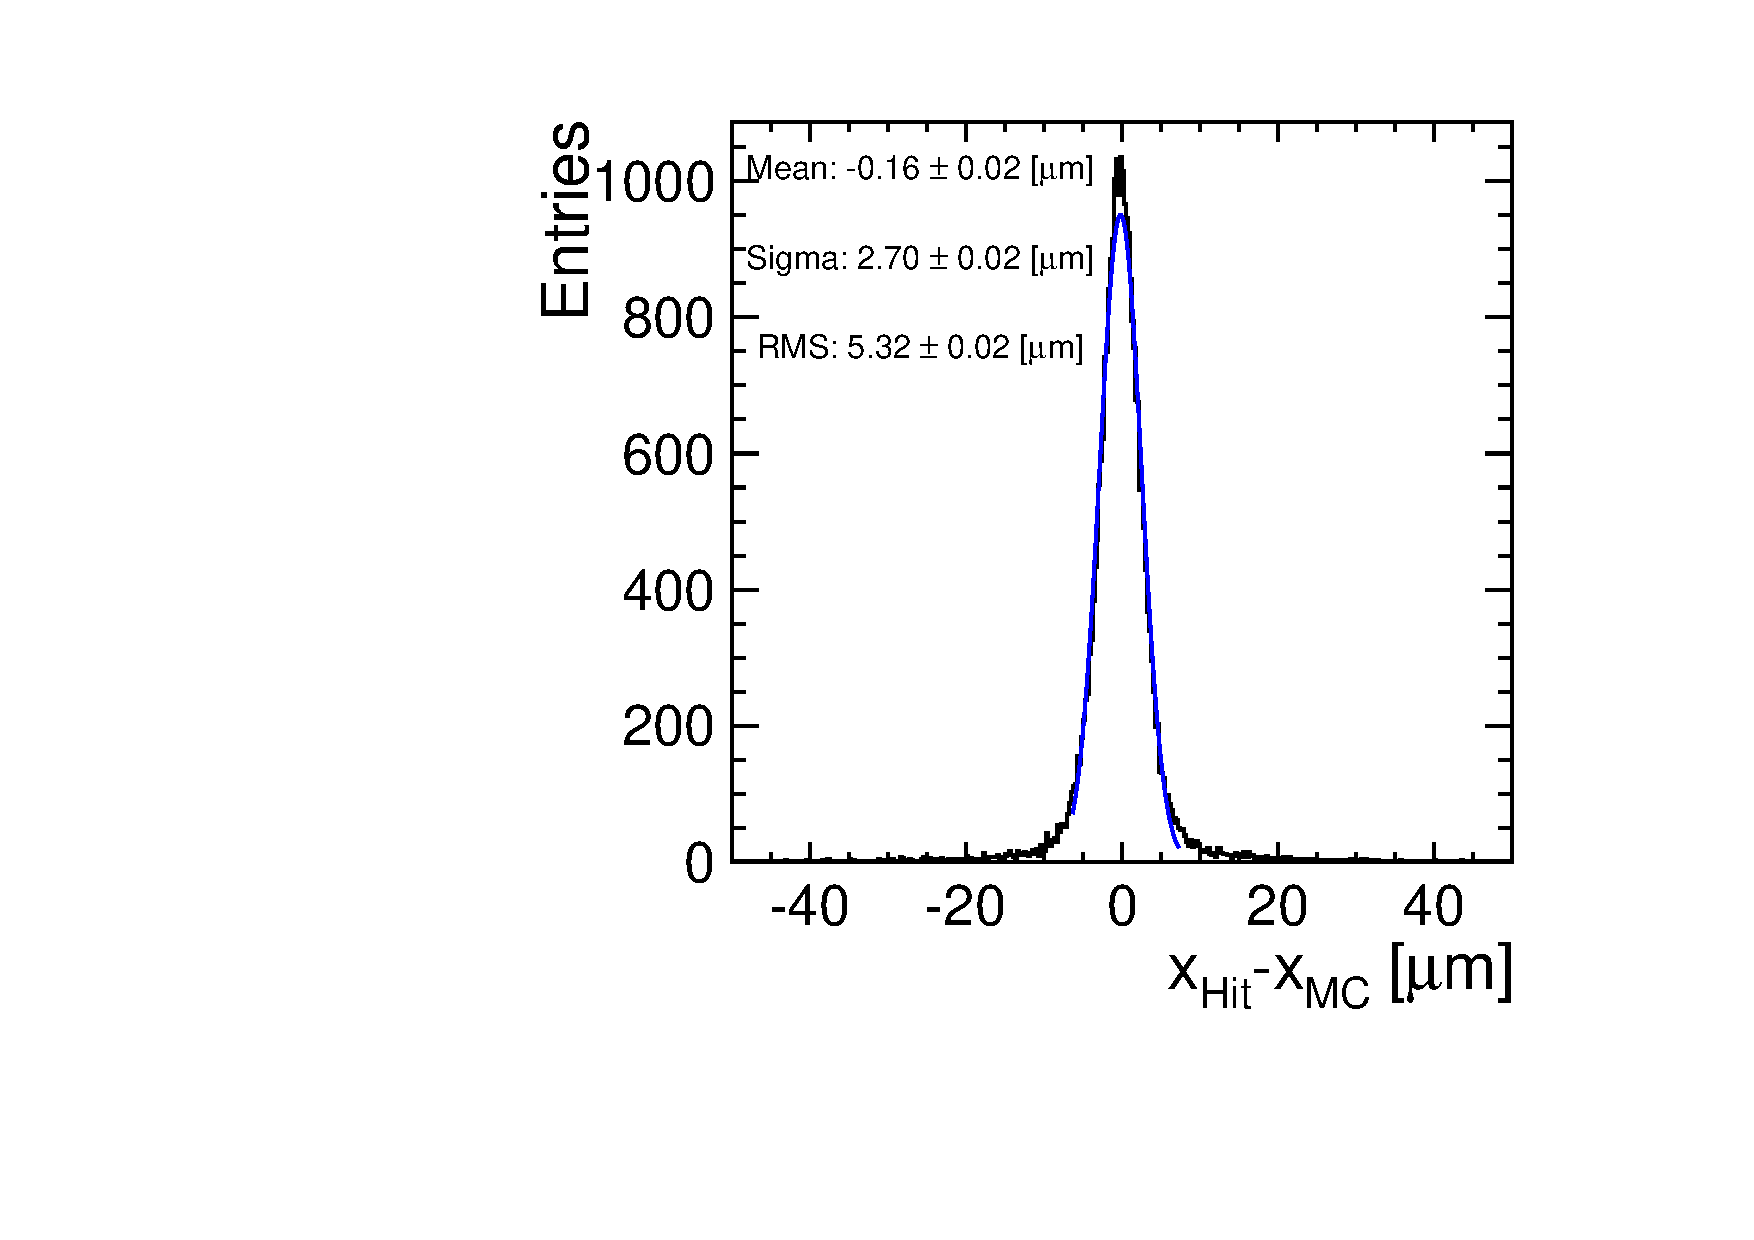
\includegraphics[width=\textwidth]{figures/Telescope/telescopePlane0_MC_vs_hit_x.pdf}
    \caption{}
  \end{subfigure}\hfill
  \begin{subfigure}[b]{0.45\textwidth}
    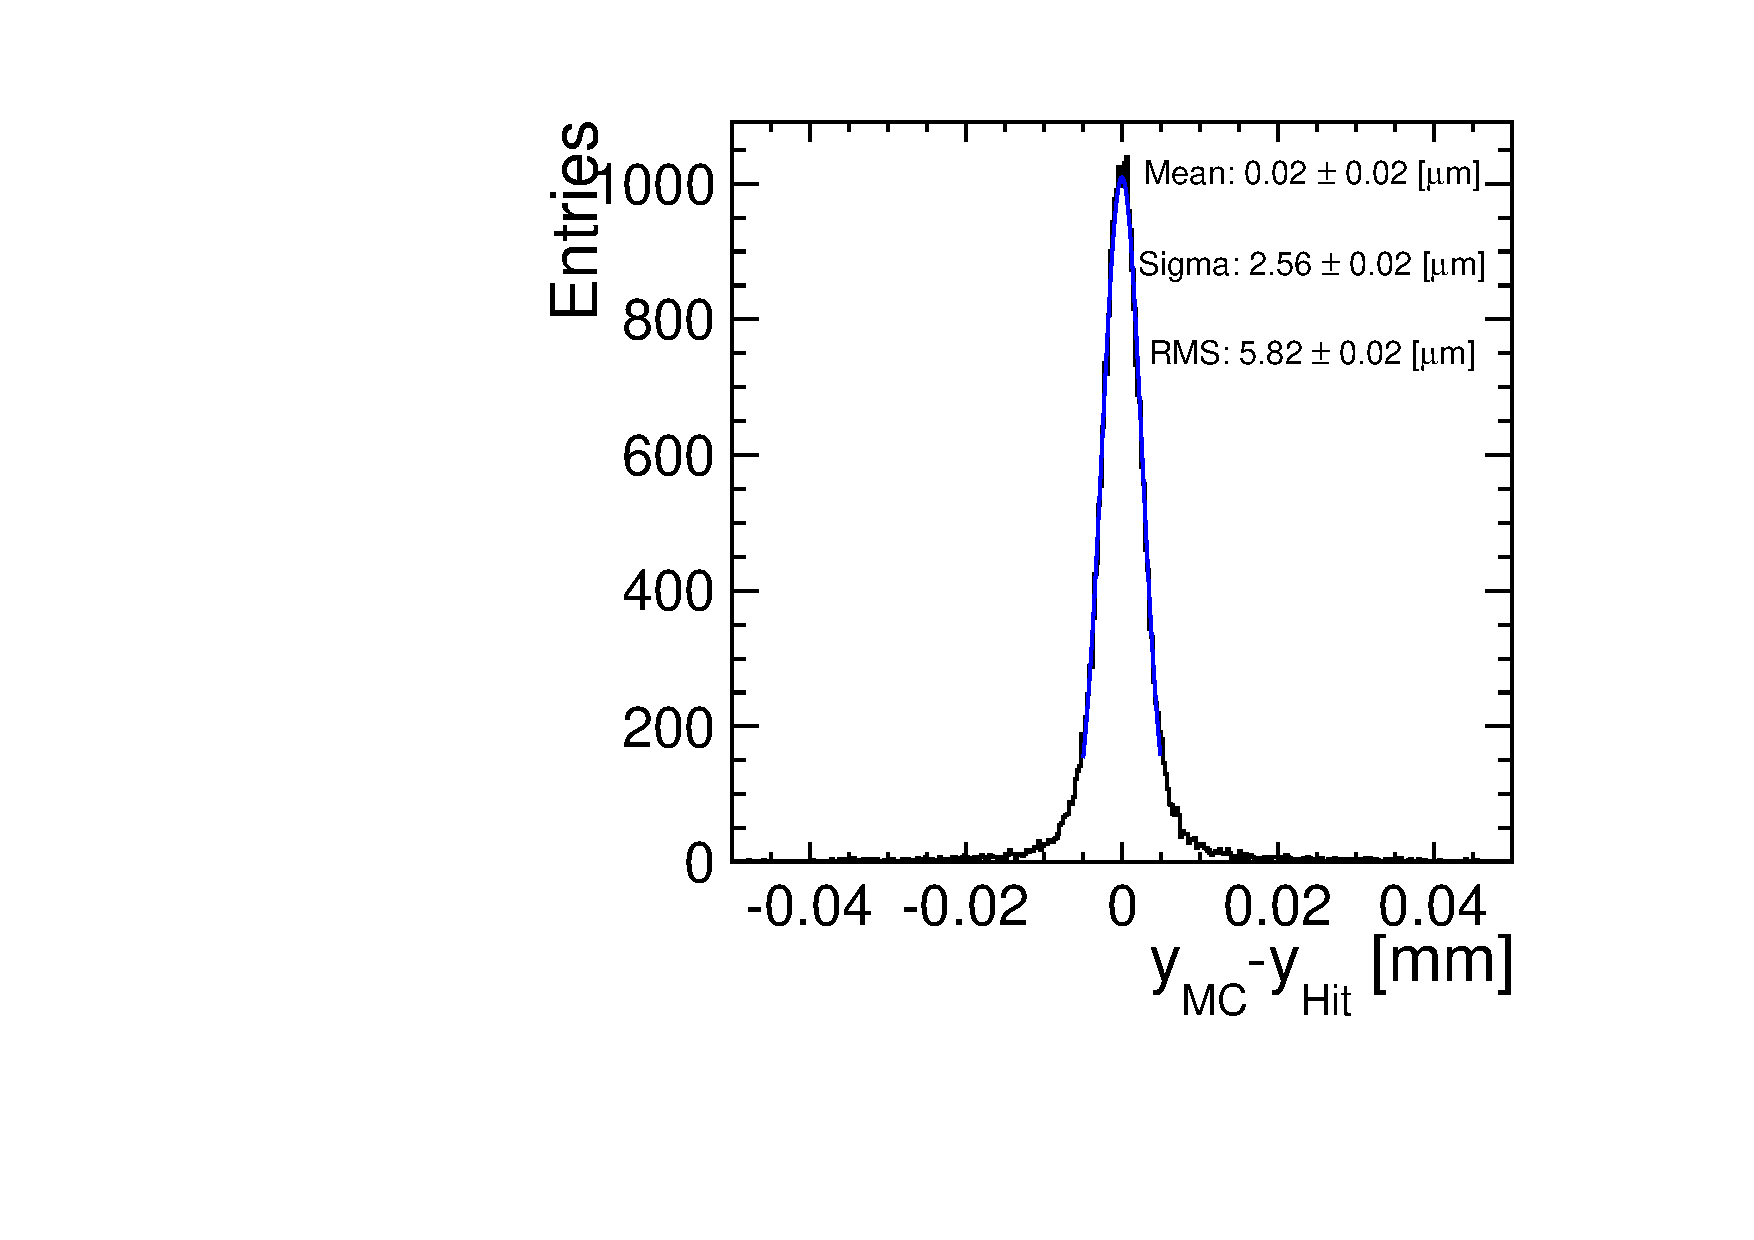
\includegraphics[width=\textwidth]{figures/Telescope/telescopePlane0_MC_vs_hit_y.pdf}
    \caption{}
  \end{subfigure}
  \caption{The intrinsic resolution of a telescope plane in (a) x and
    (b) y directions comparing the MC and the reconstructed
    hit positions.}
  \label{fig:TelPlane0_MC_hit}
\end{figure}

The residuals as a function of the x\textsubscript{MC} and
y\textsubscript{MC} are shown in \cref{fig:TelPlane0_MC_hit_2D}. The
intrinsic resolution does not depend on the position of the hit and
stays the same for all positions. This confirms the coherence between
the geometry description in the AllPix simulations and the EUTelescope
reconstruction.

\begin{figure}[htbp] \centering
  \begin{subfigure}[b]{0.45\textwidth}
    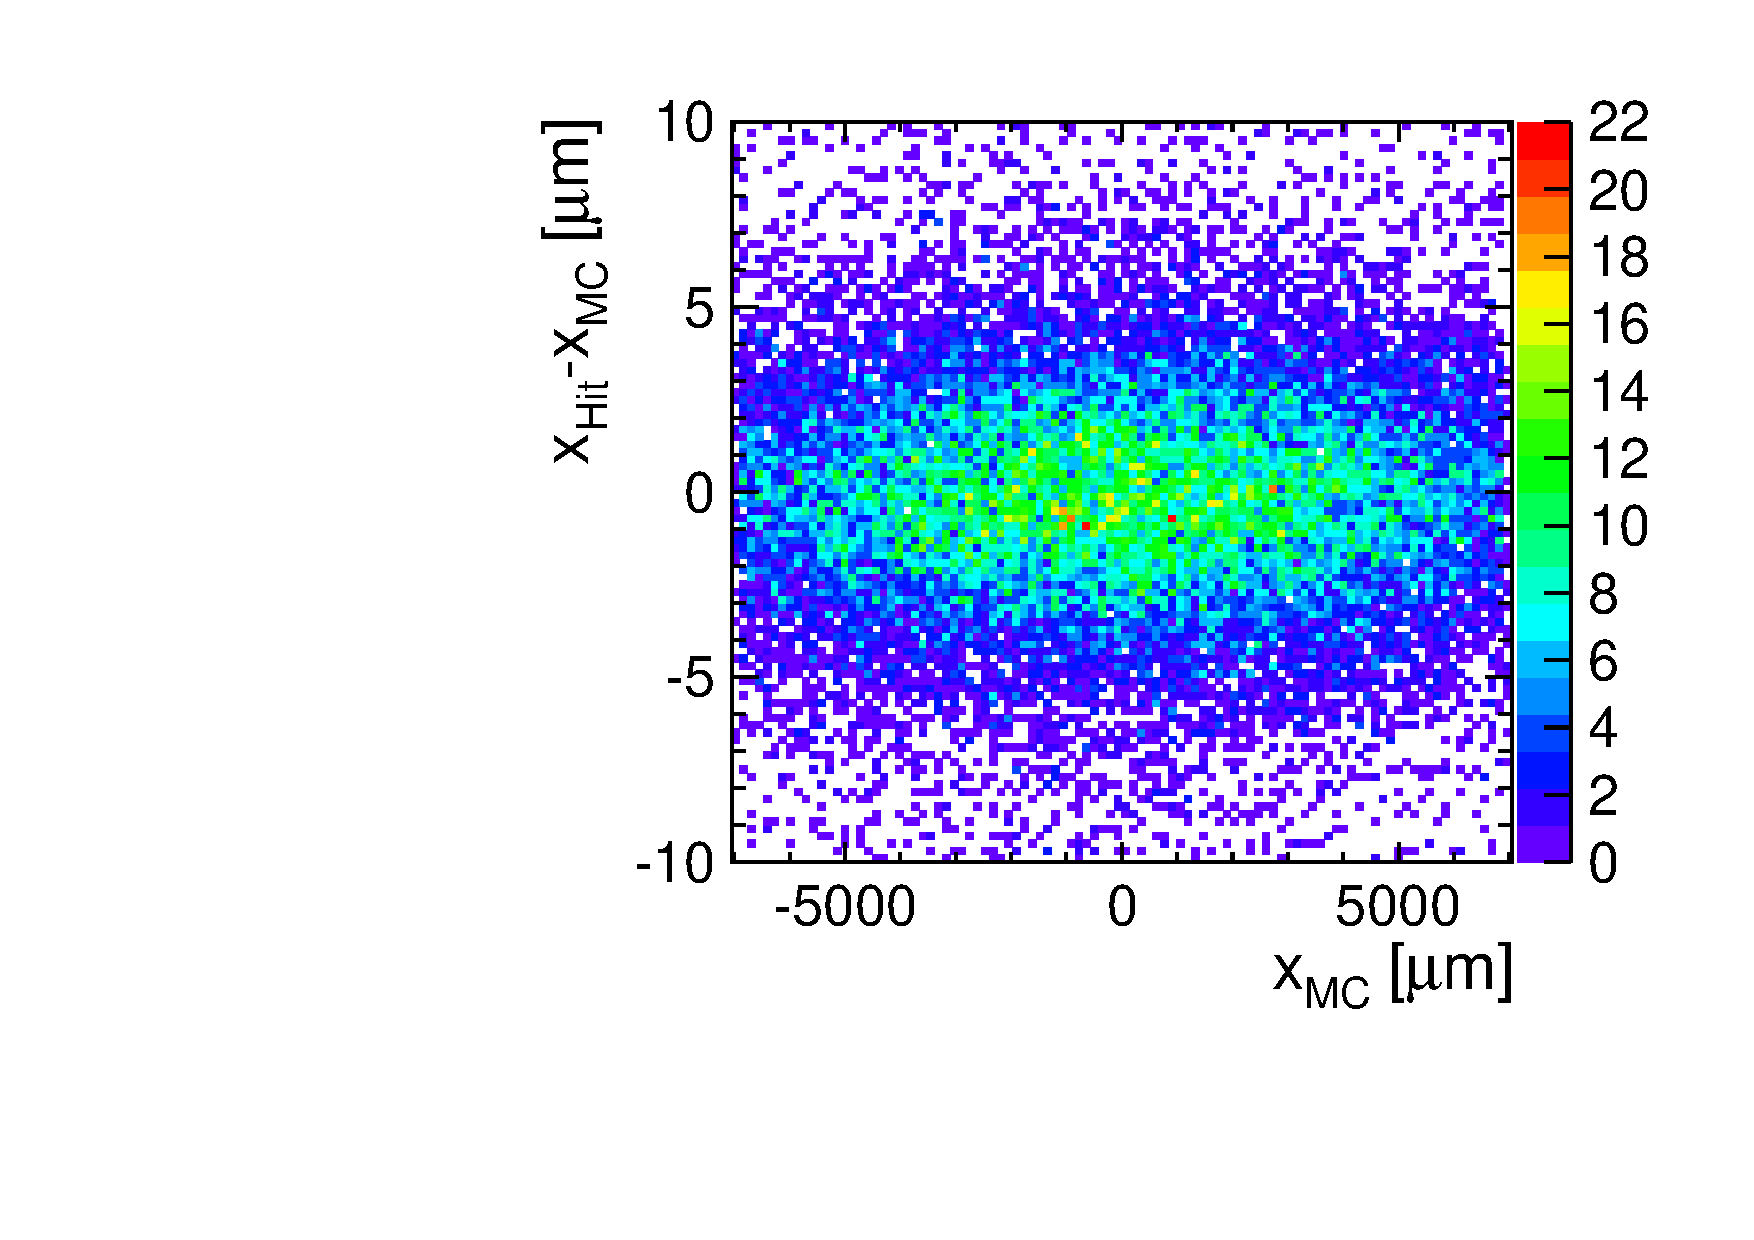
\includegraphics[width=\textwidth]{figures/Telescope/telescopePlane0_MC_vs_hit_x_2D.pdf}
    \caption{}
  \end{subfigure}\hfill
  \begin{subfigure}[b]{0.45\textwidth}
    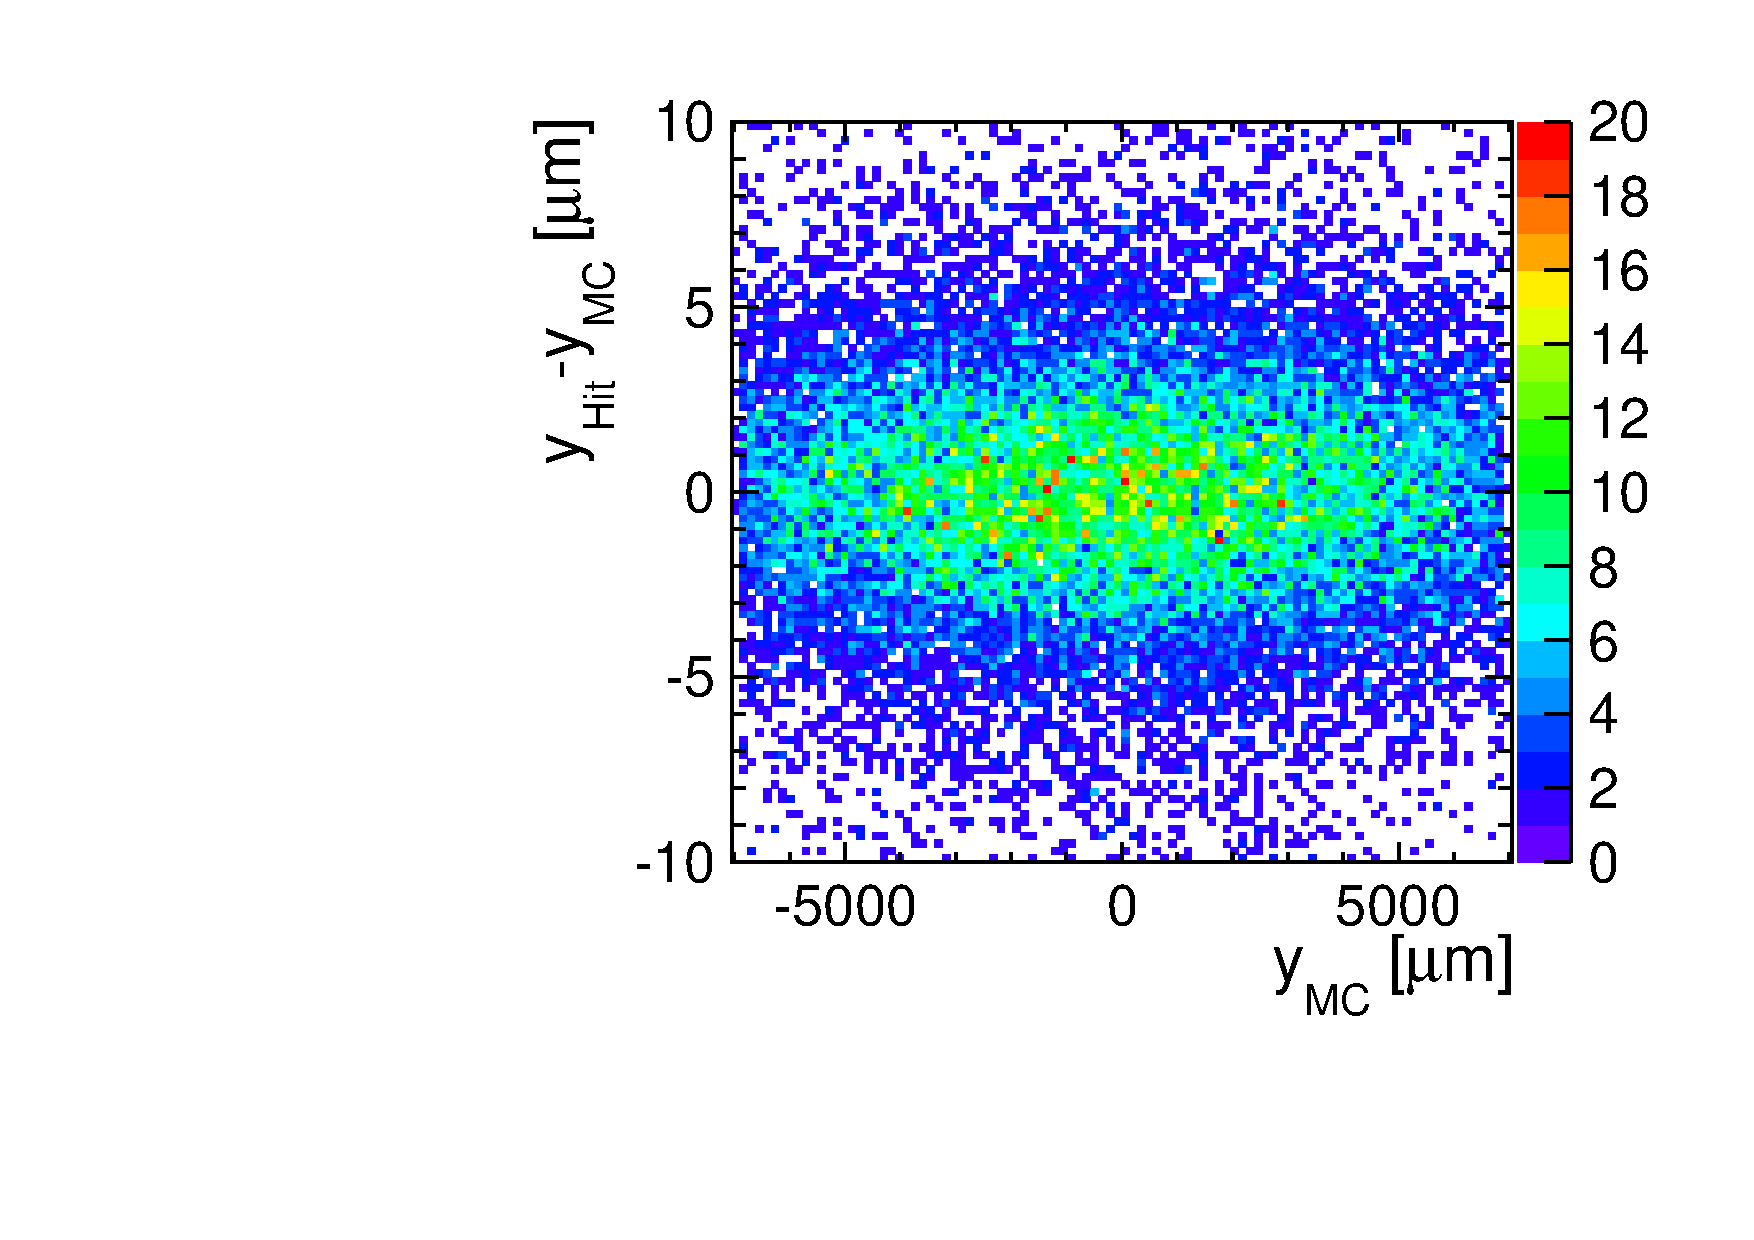
\includegraphics[width=\textwidth]{figures/Telescope/telescopePlane0_MC_vs_hit_y_2D.pdf}
    \caption{}
  \end{subfigure}
  \caption{The intrinsic resolution of a telescope plane in (a) x and
    (b) y directions comparing the MC and the reconstructed
    hit positions as a function of the MC position.}
  \label{fig:TelPlane0_MC_hit_2D}
\end{figure}


\newpage
\subsection{Biased residuals on each telescope plane}

The biased residual on each telescope plane is defined as the
difference between the measured hit and the biased fitted track
position. \cref{fig:telescopeBiasedRMS_data_simu} compares the RMS of
the biased residuals in data and simulations (the original
distributions are given in
\cref{fig:telescope_biasedResiduals_data_X,fig:telescope_biasedResiduals_data_Y}
for data and
\cref{fig:telescope_biasedResiduals_simu_X,fig:telescope_biasedResiduals_simu_Y}
for simulation). For this calculation, a cut is applied to remove
$10\%$ of tracks with the highest
$\chi^2$/NDF. \cref{fig:chi2_data_simu} shows the $\chi^2$/NDF in data
(a) and in simulations (b) with a cut applied illustrated in a red
line.
\begin{figure}[htbp] \centering
  \begin{subfigure}[b]{0.45\textwidth}
    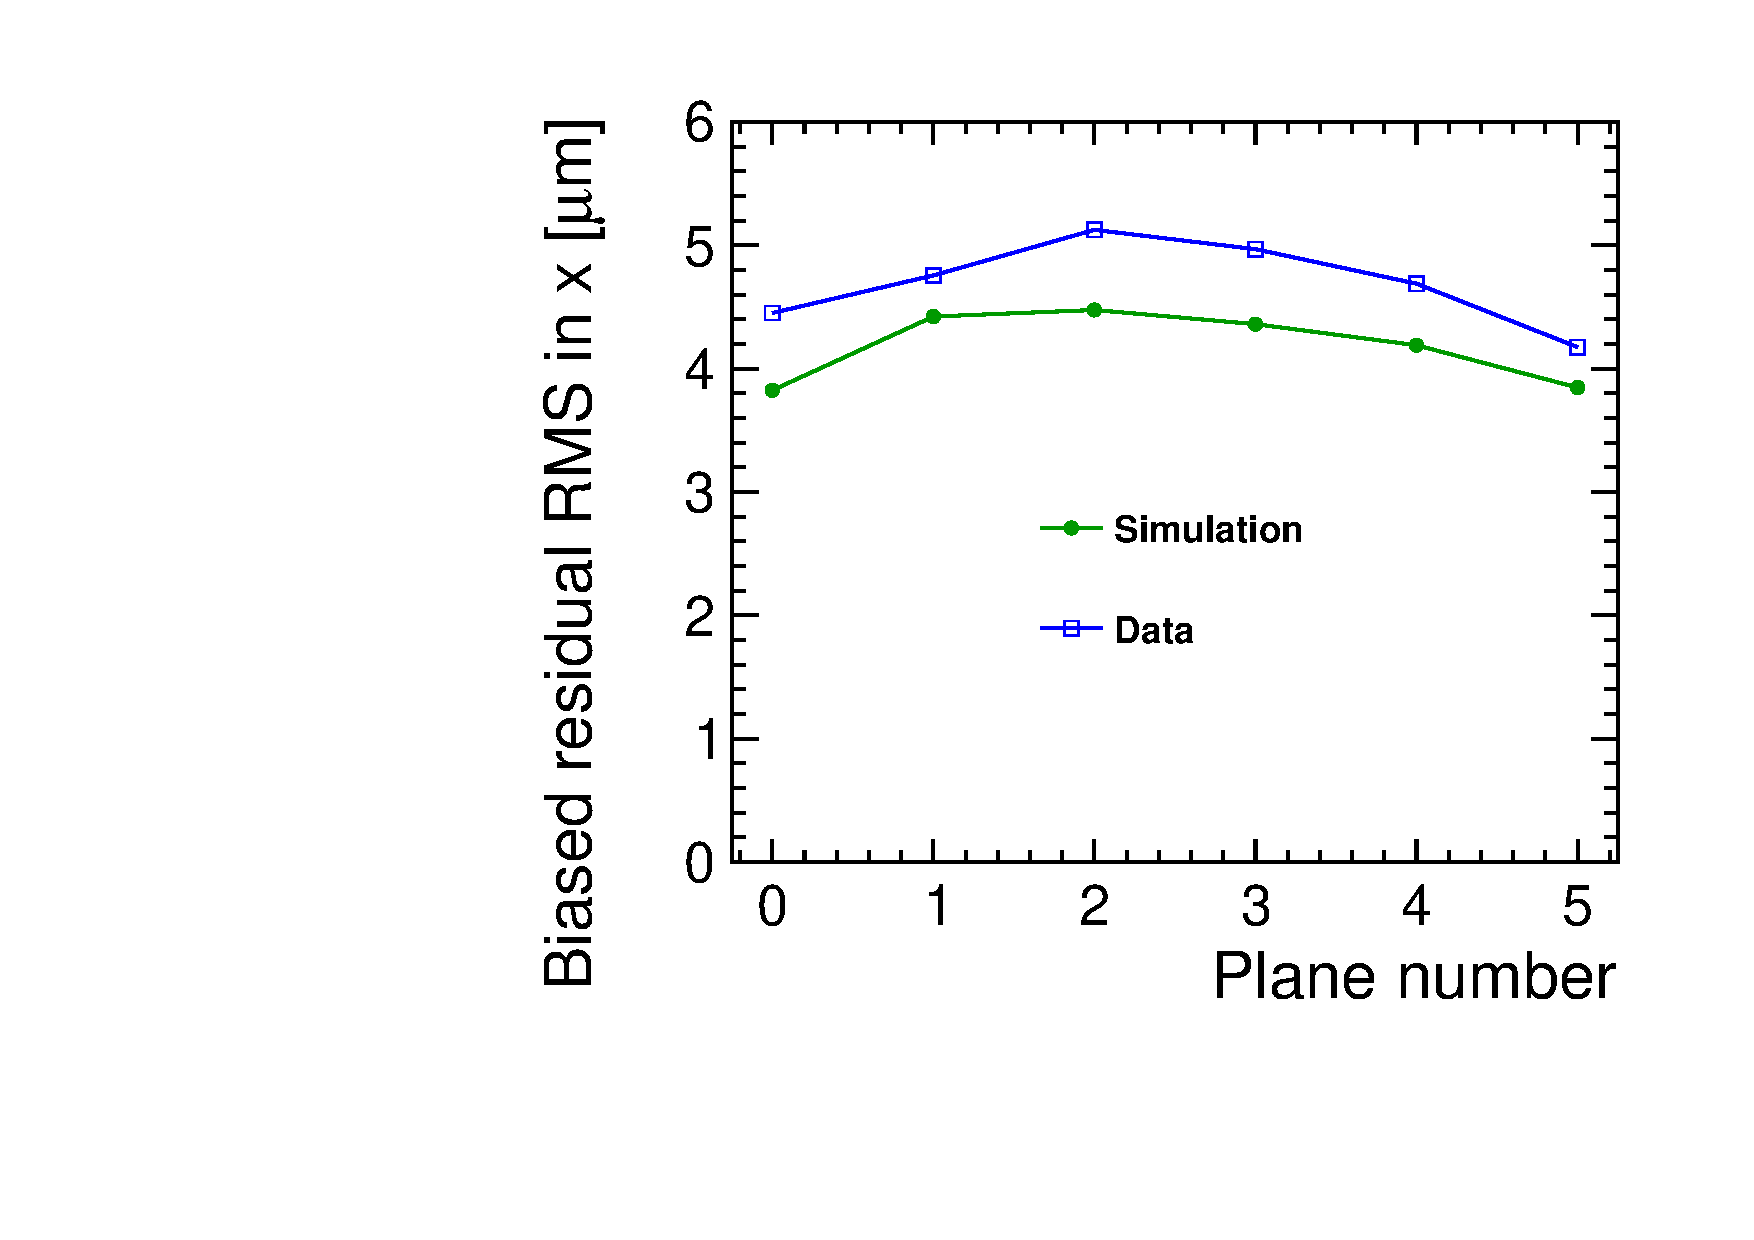
\includegraphics[width=\textwidth]{figures/Telescope/biasedResiduals/RMSX_simu_vs_data.pdf}
    \caption{}
  \end{subfigure}\hfill
  \begin{subfigure}[b]{0.45\textwidth}
    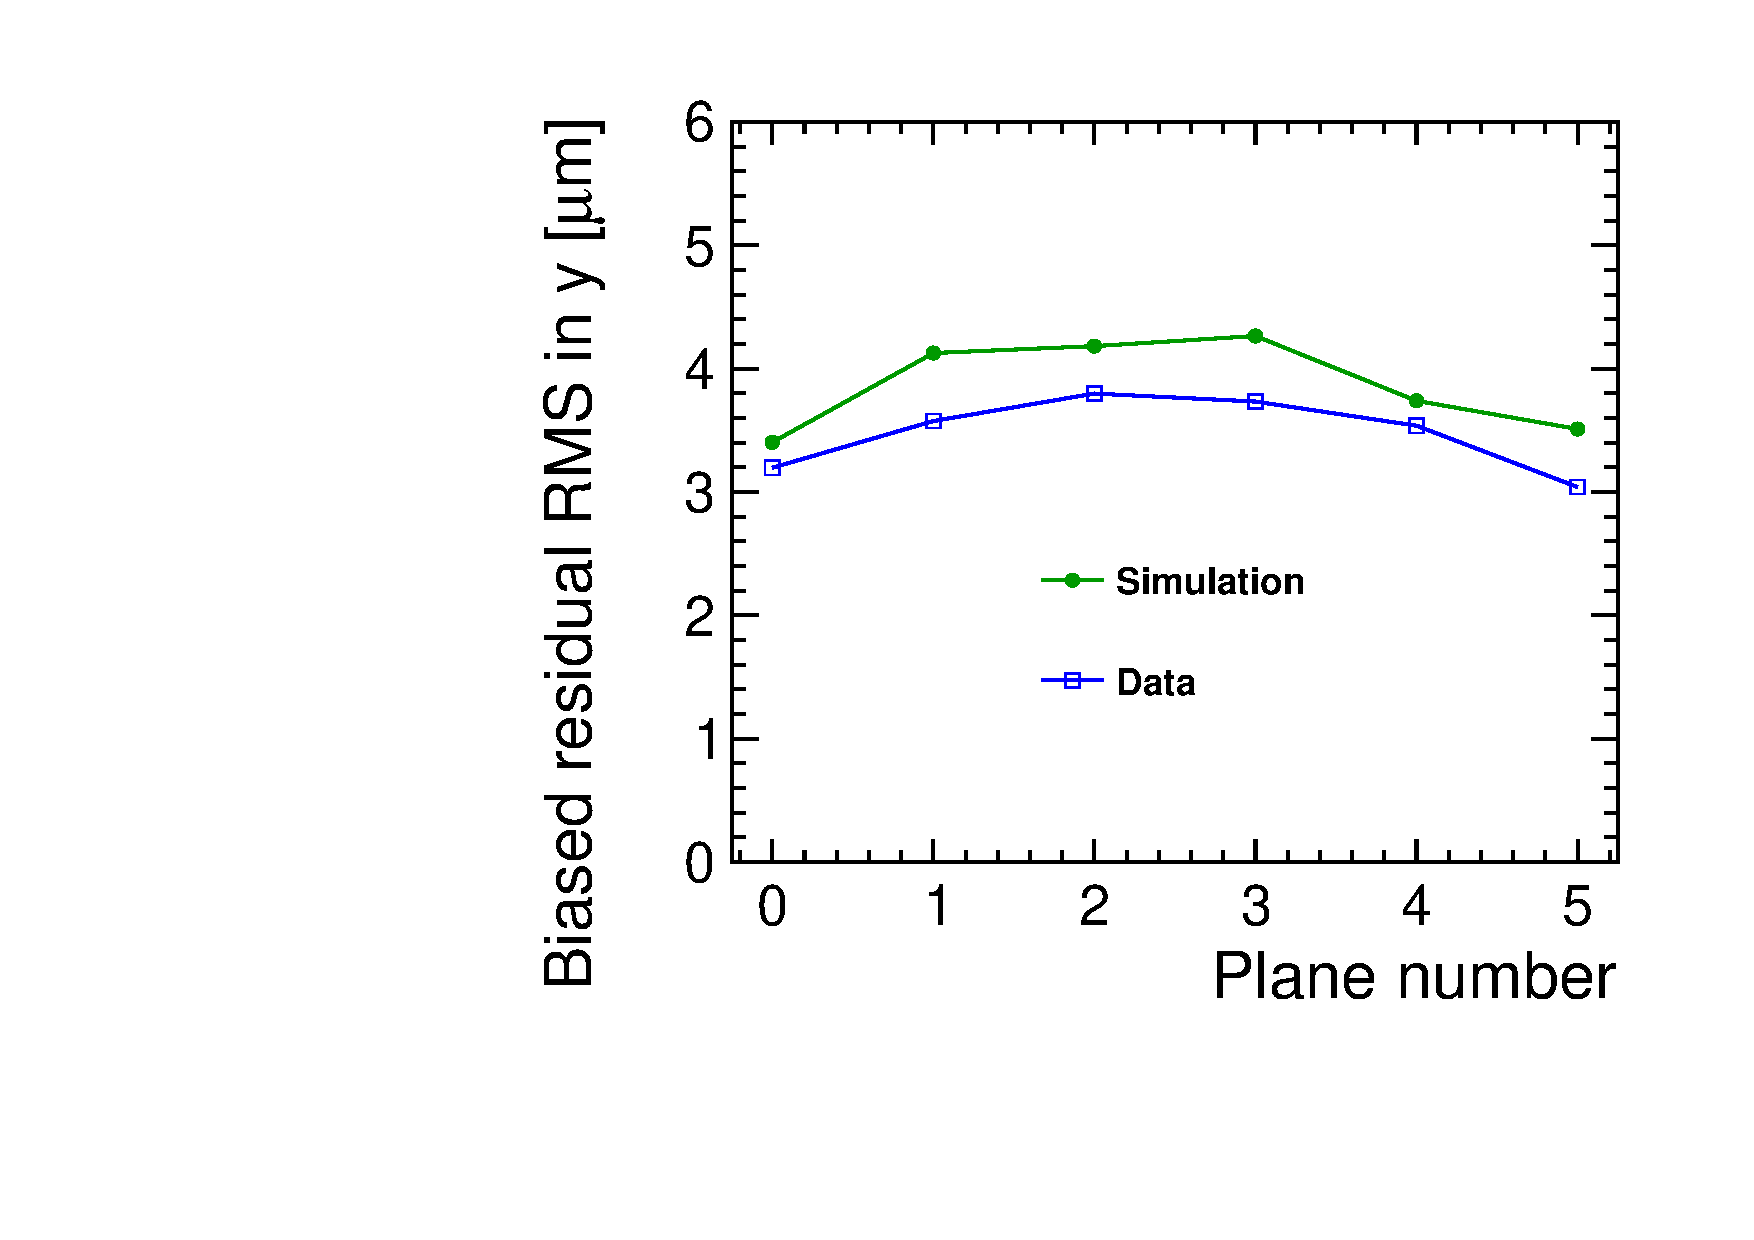
\includegraphics[width=\textwidth]{figures/Telescope/biasedResiduals/RMSY_simu_vs_data.pdf}
    \caption{}
  \end{subfigure}
  \caption{The RMS of the biased residuals in the (a) x and (b) y directions
    comparing the data and simulation for the telescope planes. A cut
    is applied to remove the $10\%$ of tracks with highest
    $\chi^2$/NDF.}
  \label{fig:telescopeBiasedRMS_data_simu}
\end{figure}


\begin{figure}[htbp] \centering
  \begin{subfigure}[b]{0.45\textwidth}
    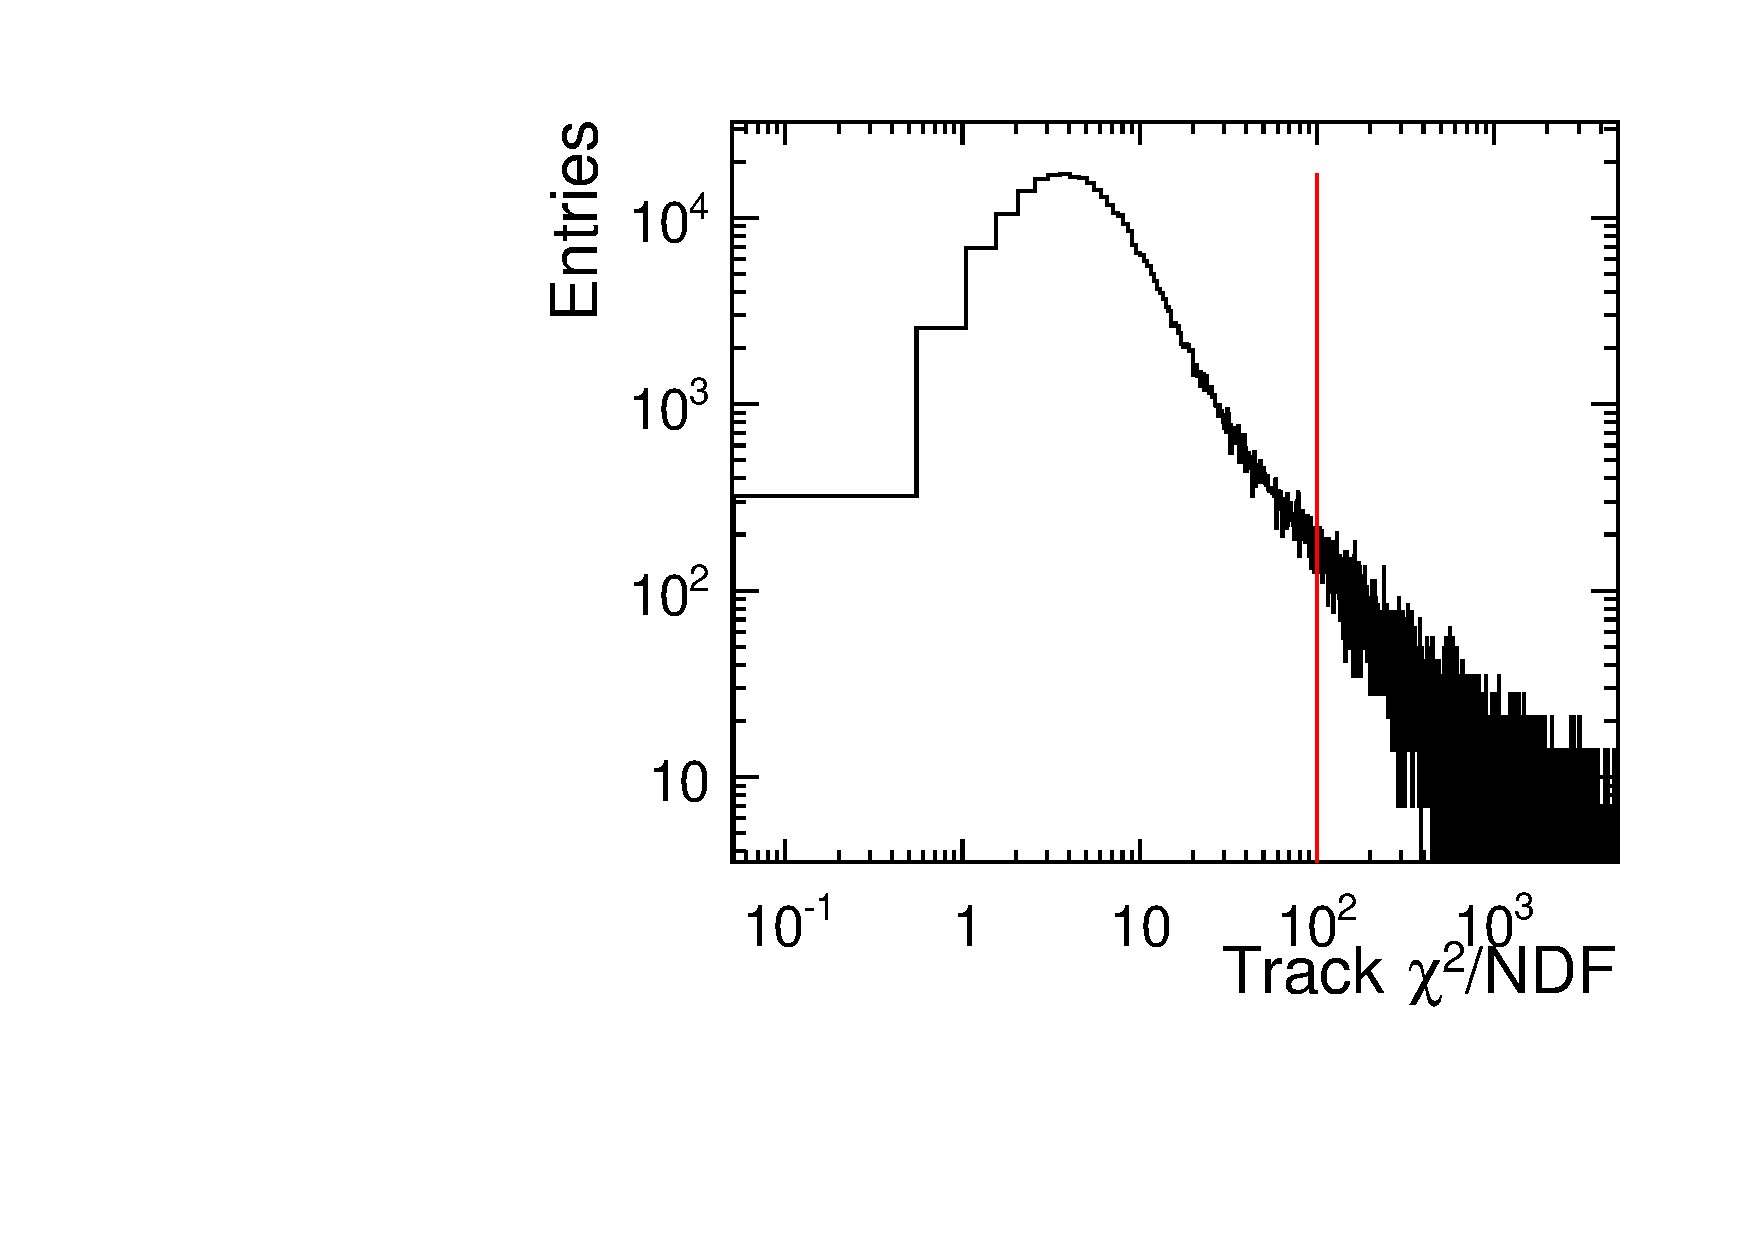
\includegraphics[width=\textwidth]{figures/Telescope/biasedResiduals/chi2_run661.pdf}
    \caption{Data}
  \end{subfigure}\hfill
  \begin{subfigure}[b]{0.45\textwidth}
    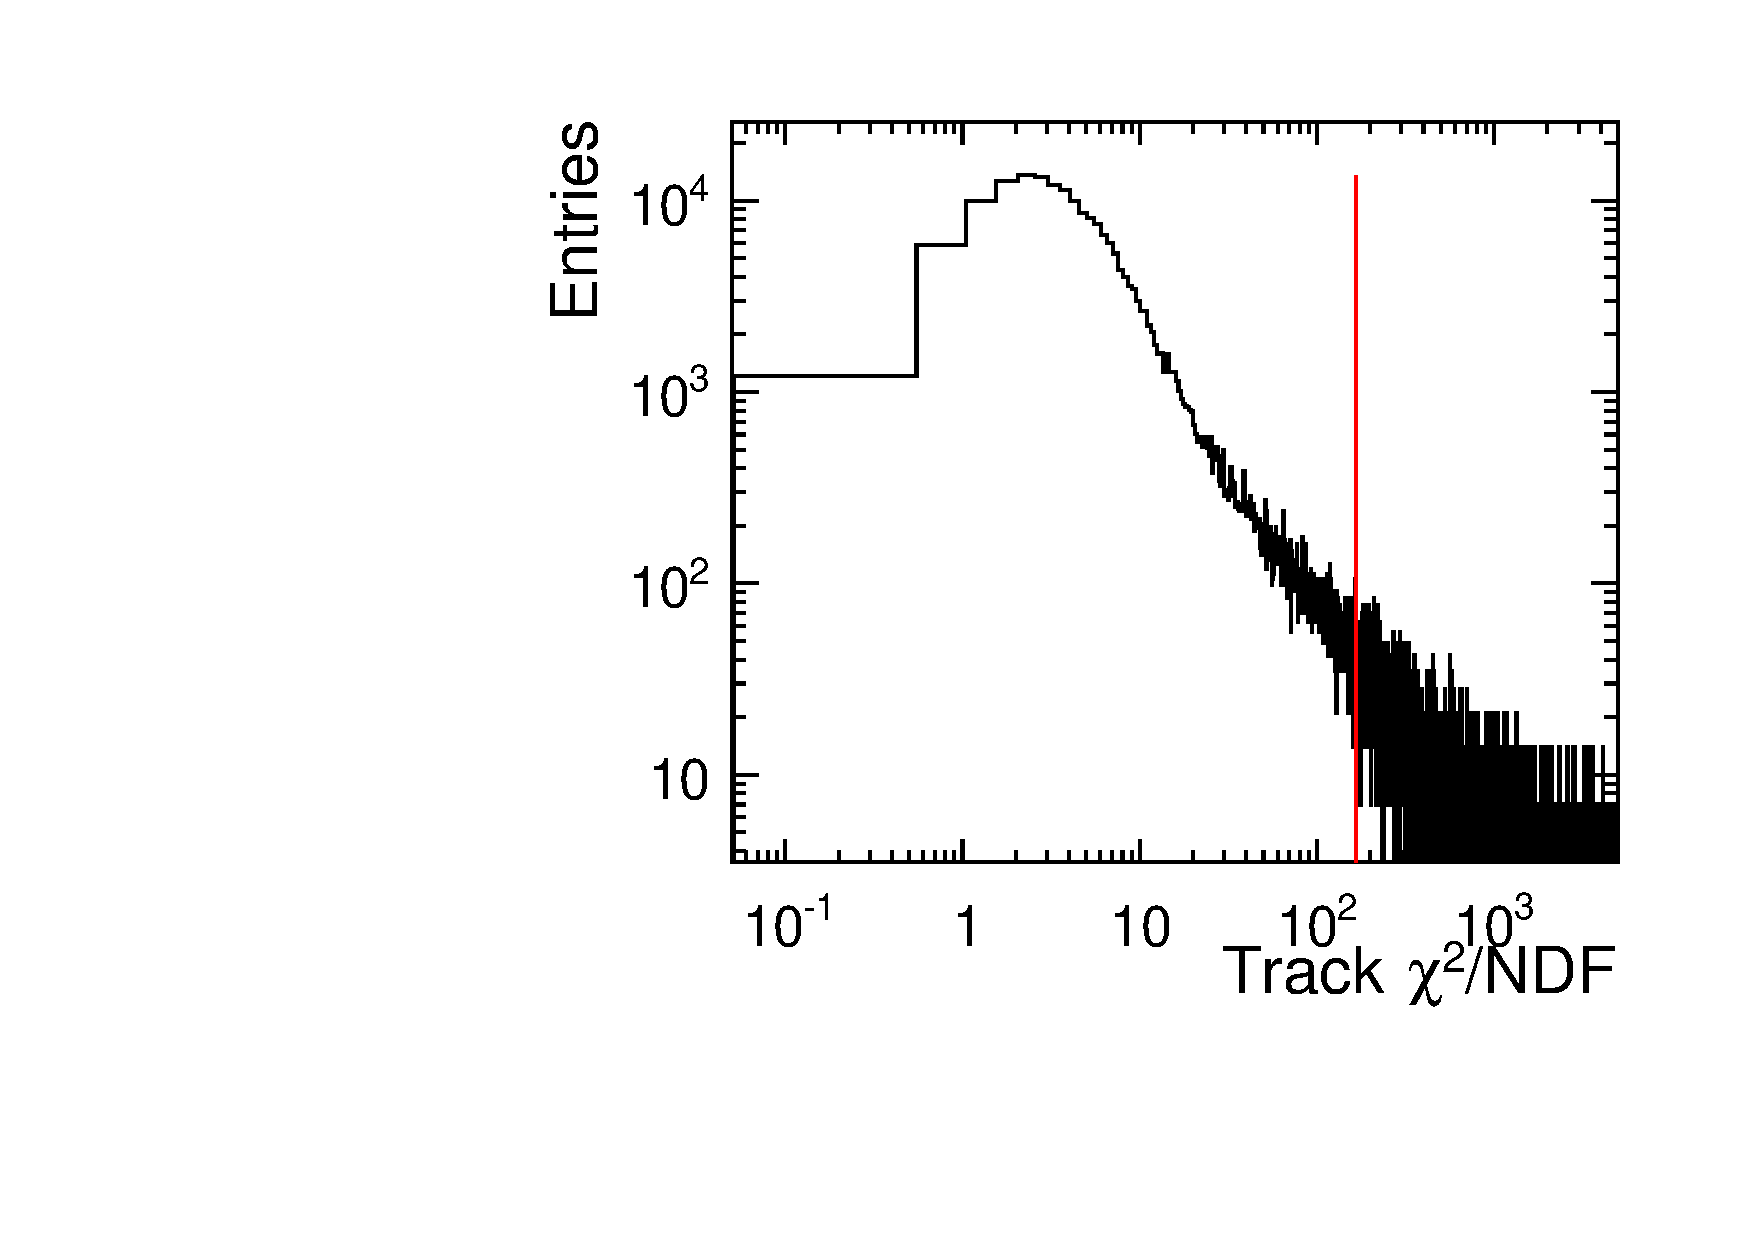
\includegraphics[width=\textwidth]{figures/Telescope/biasedResiduals/chi2_run77.pdf}
    \caption{Simulation}
  \end{subfigure}
  \caption{$\chi^2$/NDF distributions for (a) data and (b)
    simulation. A cut is applied to remove the $10\%$ of tracks with
    highest $\chi^2$/NDF (at the position of the red line).}
  \label{fig:chi2_data_simu}
\end{figure}

The width of the biased residuals increases with the distance (in z
direction). In fact, the uncertainty on the deflection angle due to
the multiple scatterings increases with larger distances of the
telescope planes.



\subsection{Tracking resolution on the DUT}
The tracking resolution on the DUT ($100\,\micron$ thick sensor) in
the x and y directions is shown in \cref{fig:DUT_MC_track}. This value
can be only obtained in simulations as the MC position is
needed.

\begin{figure}[htbp] \centering
  \begin{subfigure}[b]{0.45\textwidth}
    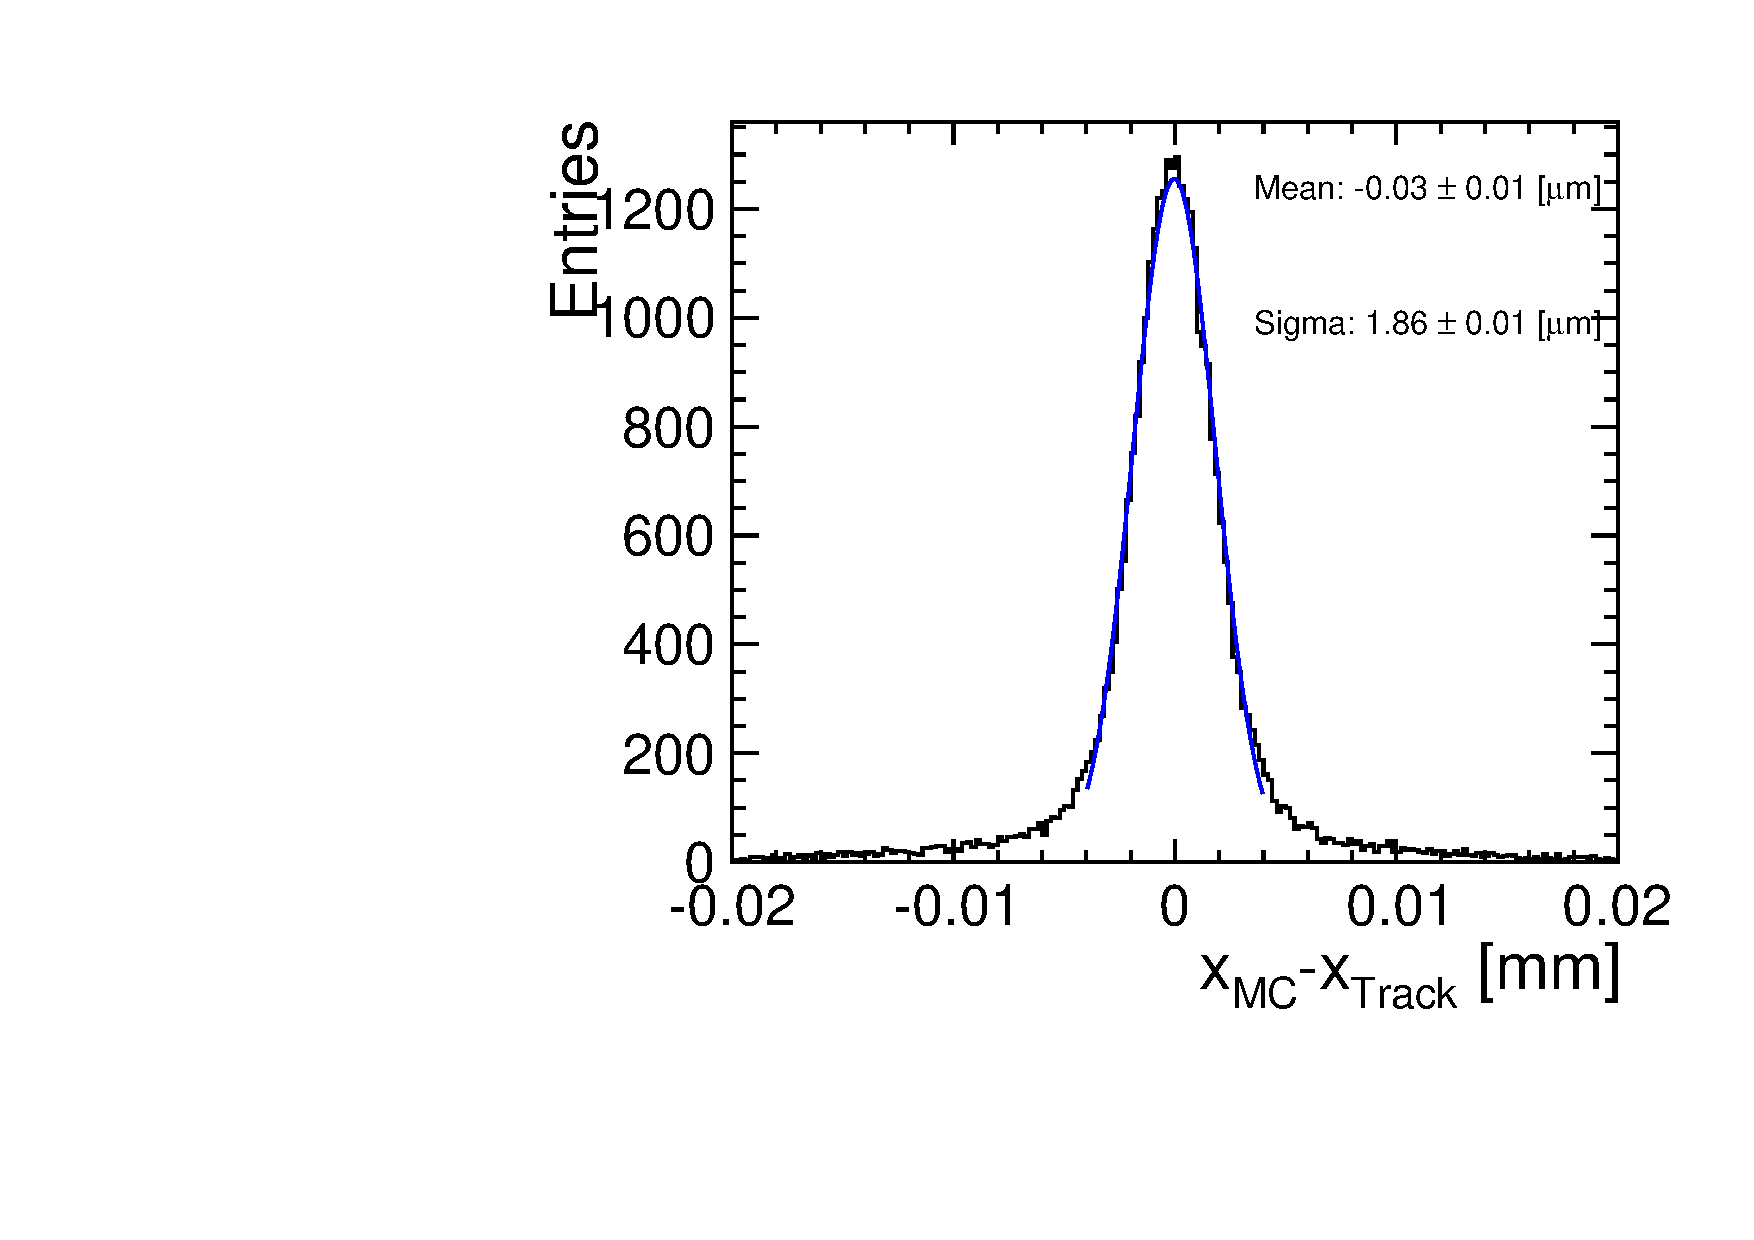
\includegraphics[width=\textwidth]{figures/Telescope/Unbiased_trackRes_DUT_x.pdf}
    \caption{}
  \end{subfigure}\hfill
  \begin{subfigure}[b]{0.45\textwidth}
    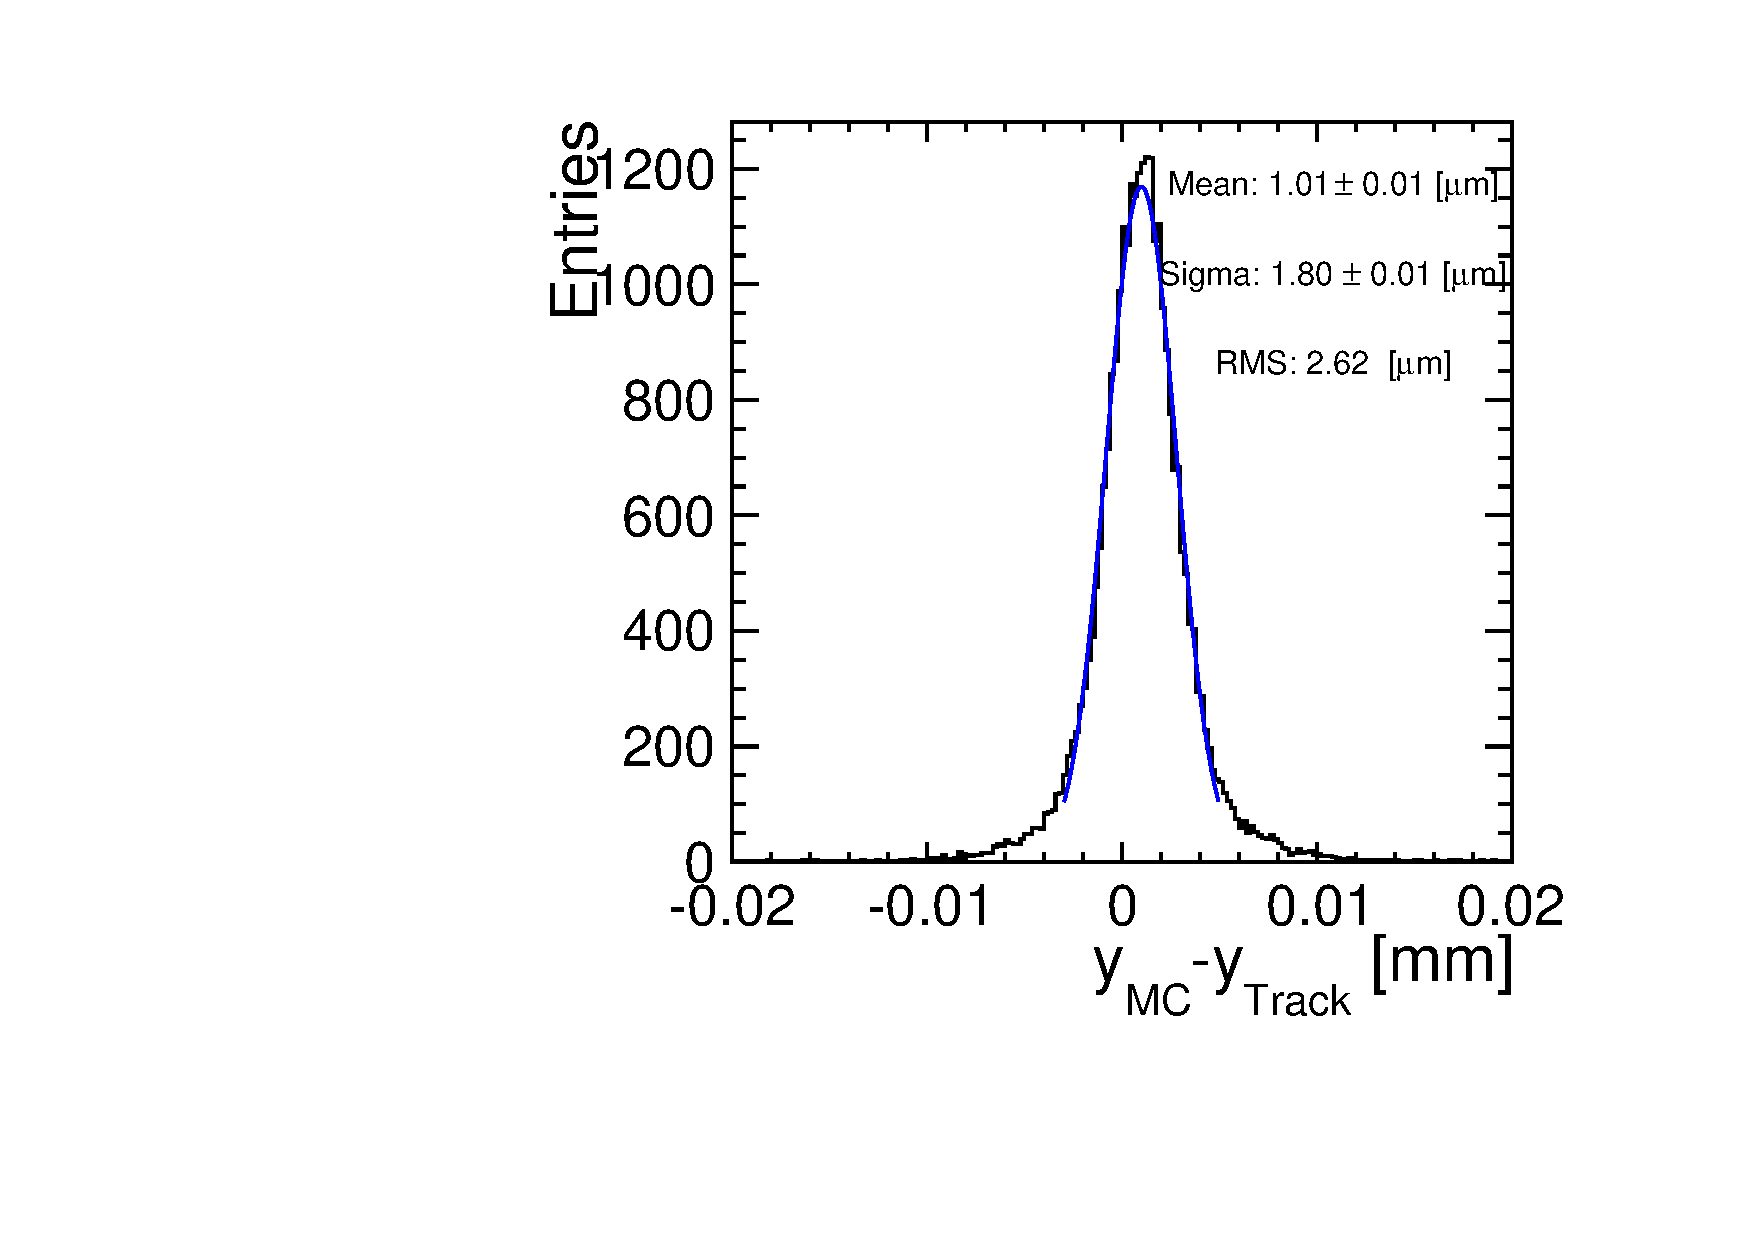
\includegraphics[width=\textwidth]{figures/Telescope/Unbiased_trackRes_DUT_y.pdf}
    \caption{}
  \end{subfigure}
  \caption{The tracking resolution on the DUT comparing the
    reconstructed track position to the true position of the particles
    obtained from \textsc{Geant4} in AllPix simulations in (a) x and
    (b) y directions.}
  \label{fig:DUT_MC_track}
\end{figure}


The tracking resolution on the DUT as a function of the
x\textsubscript{MC} and y\textsubscript{MC} positions is shown in
\cref{fig:DUT_MC_track_2D}.

\begin{figure}[htbp] \centering
  \begin{subfigure}[b]{0.45\textwidth}
    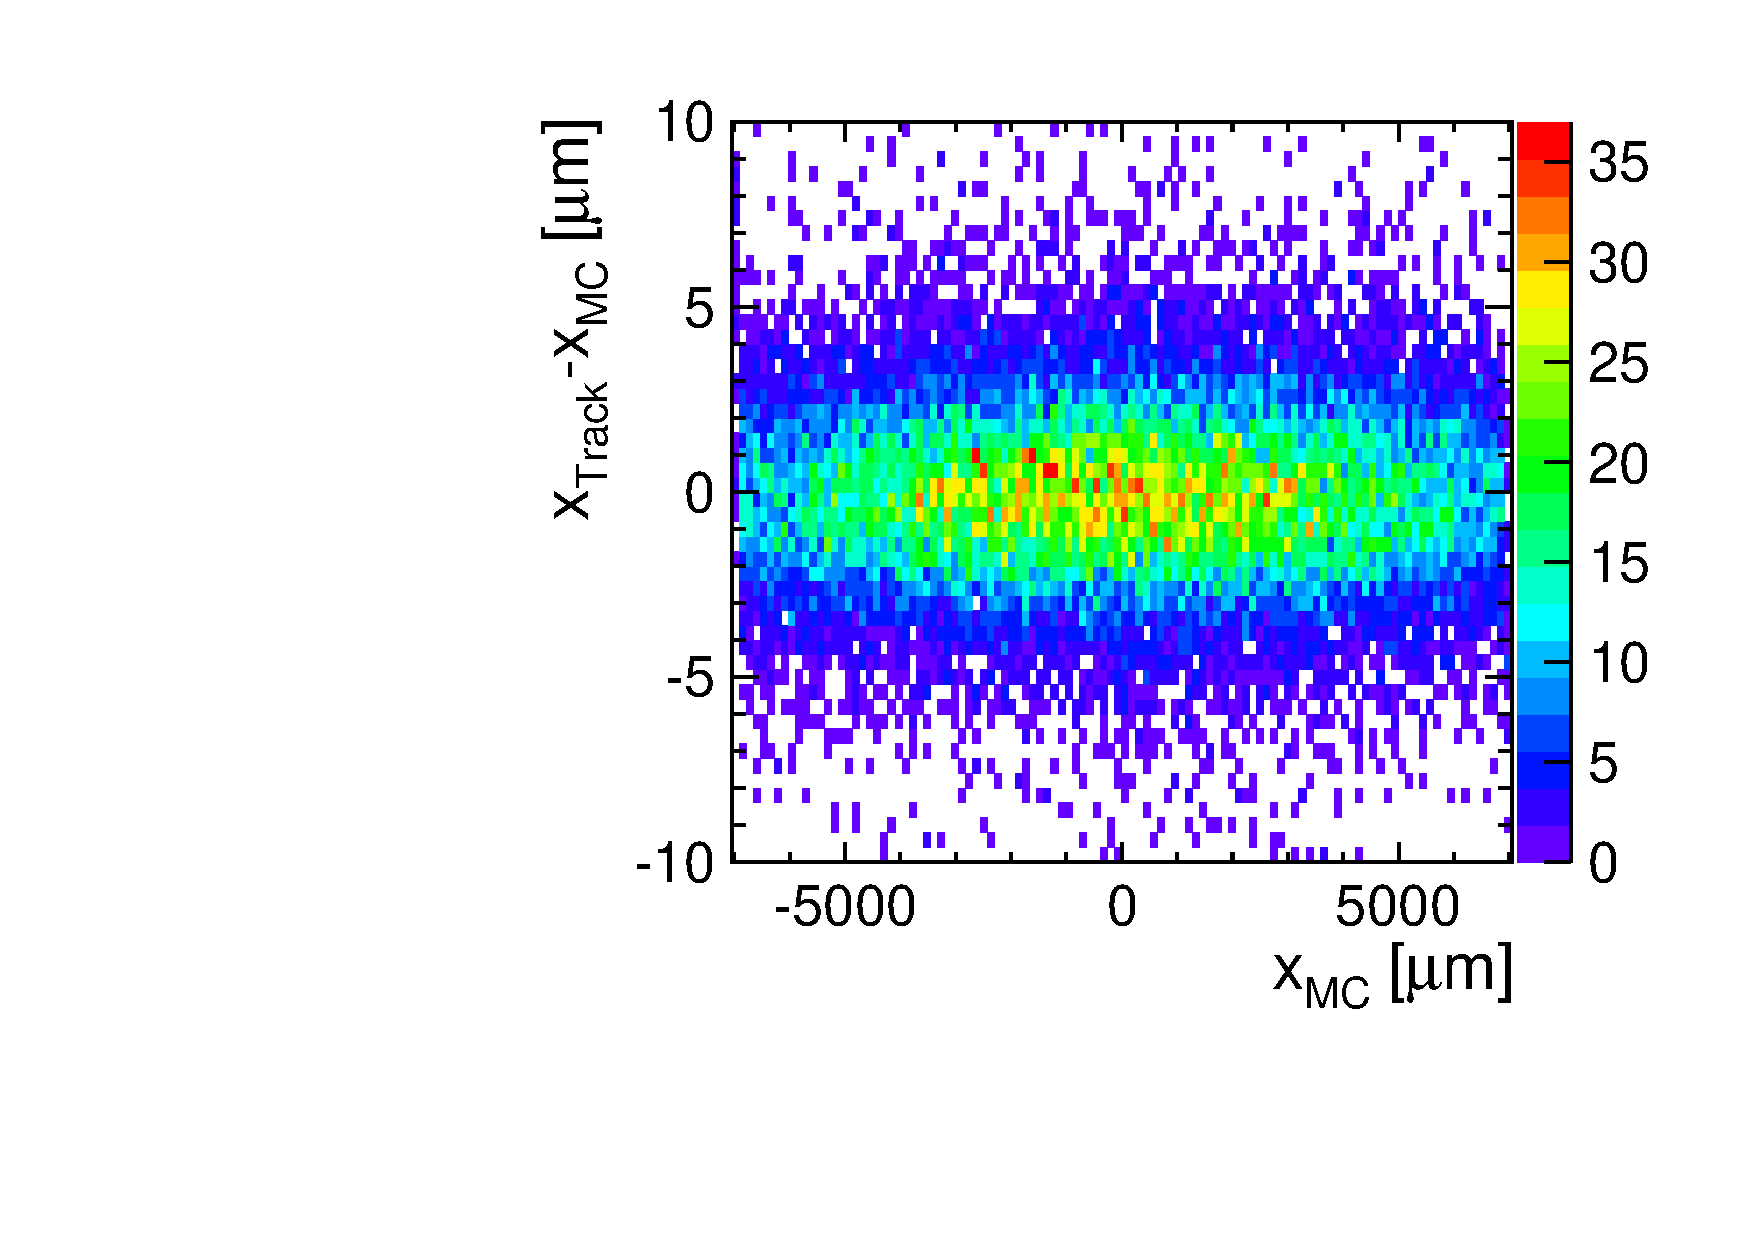
\includegraphics[width=\textwidth]{figures/Telescope/Unbiased_trackRes_DUT_x_2D.pdf}
    \caption{}
  \end{subfigure}\hfill
  \begin{subfigure}[b]{0.45\textwidth}
    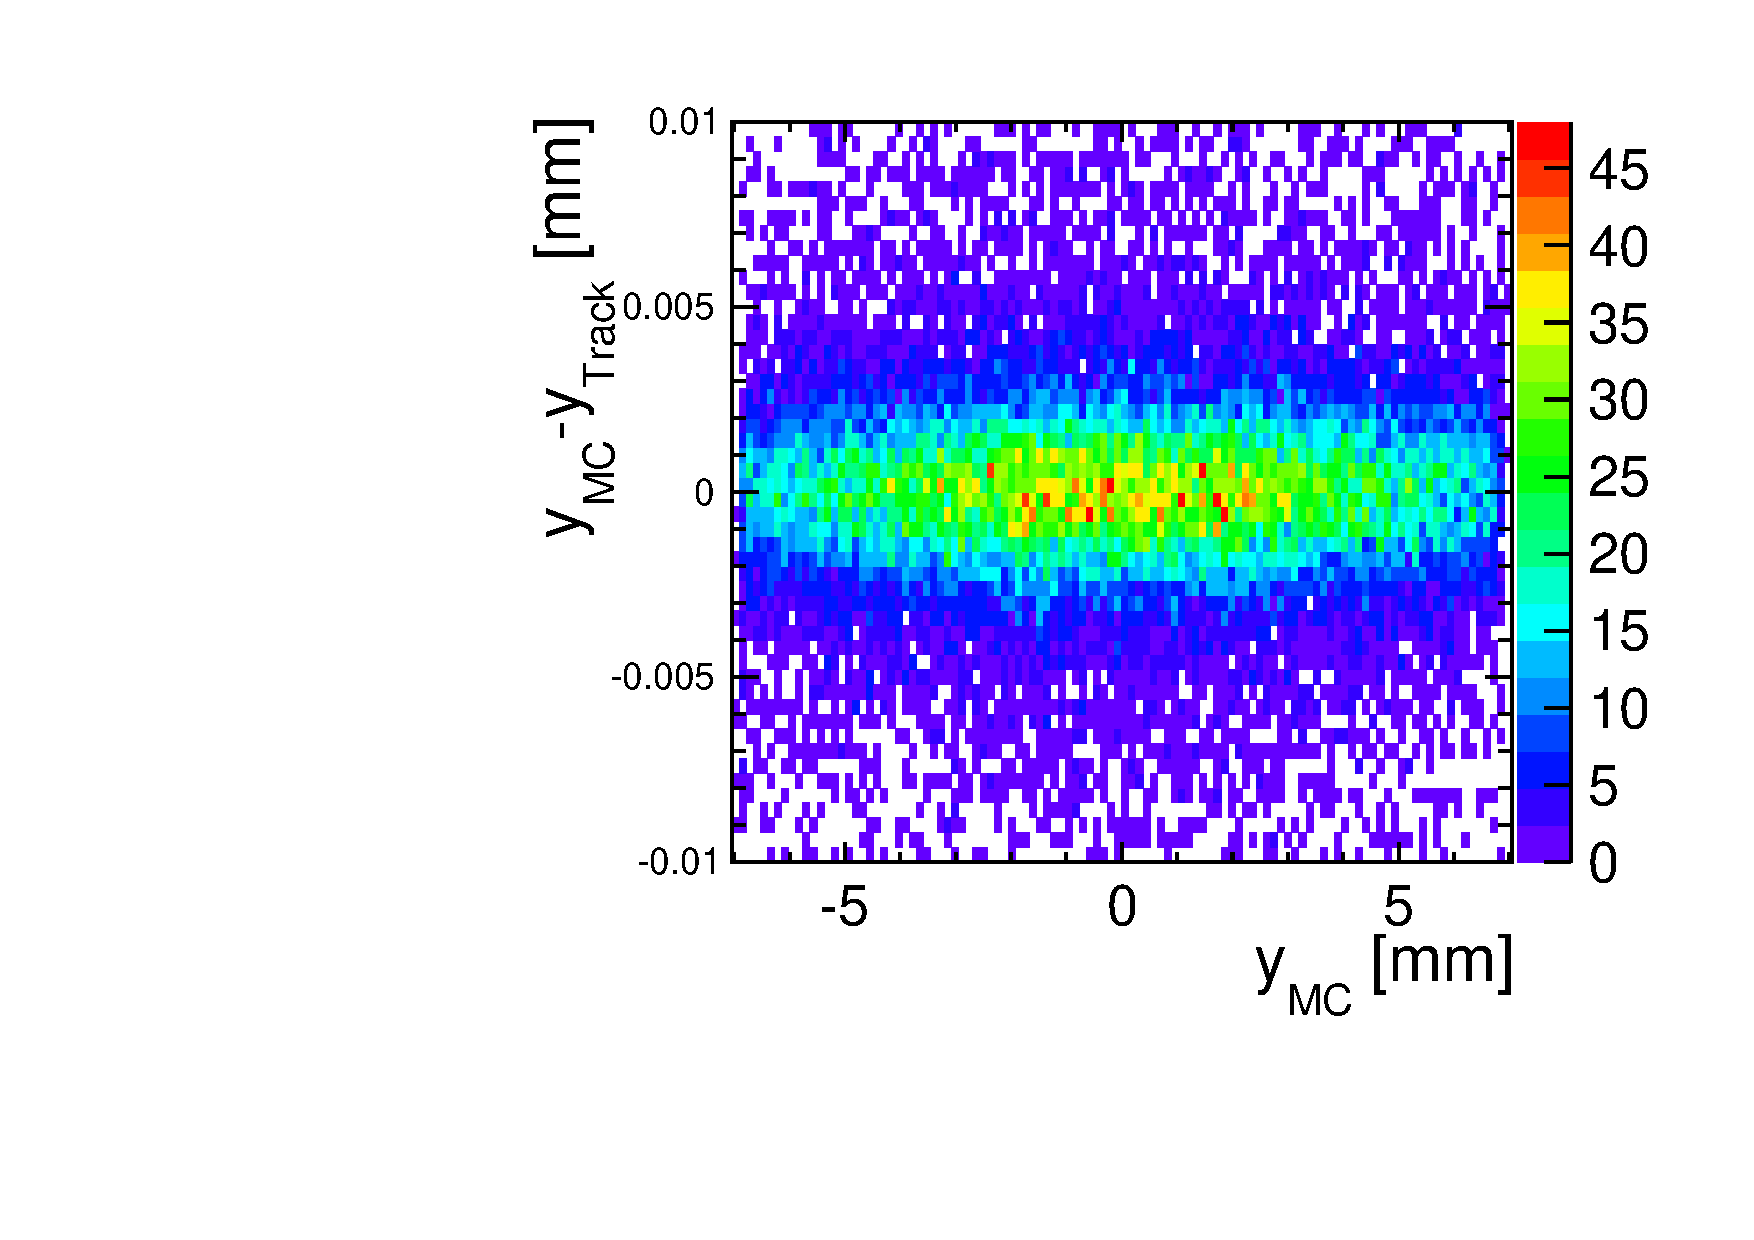
\includegraphics[width=\textwidth]{figures/Telescope/Unbiased_trackRes_DUT_y_2D.pdf}
    \caption{}
  \end{subfigure}
  \caption{The tracking resolution on the DUT in (a) x and (b)
    directions as a function of the MC position.}
  \label{fig:DUT_MC_track_2D}
\end{figure}

\cref{tab:SummaryOfResolutions} summarises the telescope resolutions
measured by the simulations.

\begin{table}[htbp]
  \centering
  \caption{A summary of the measured telescope performance.}
  \label{tab:SummaryOfResolutions}
  \begin{tabular}{ccc}
    \toprule
    $\sigma$\textsubscript{int} [$\micron$] & $\sigma$\textsubscript{x,DUT} [$\micron$] & $\sigma$\textsubscript{y,DUT} [$\micron$]\\
    \midrule
    2.4 & 1.86 & 1.60 \\
    \bottomrule
  \end{tabular}
\end{table}


%% --------------------------------------------- %%

\subsection{Beam angle}

For MC beam angle distribution:

\begin{equation}
  \phi=arctan{{x_2-x_{DUT}} \over {z_2-z_{DUT}}} \; ,
  \label{eq:beamAnglePhi}
\end{equation}

\begin{equation}
  \theta=arctan{{y_2-y_{DUT}} \over {z_2-z_{DUT}}} \; ,
  \label{eq:beamAngleTheta}
\end{equation}

\begin{figure}[htbp] \centering
  \begin{subfigure}[b]{0.45\textwidth}
    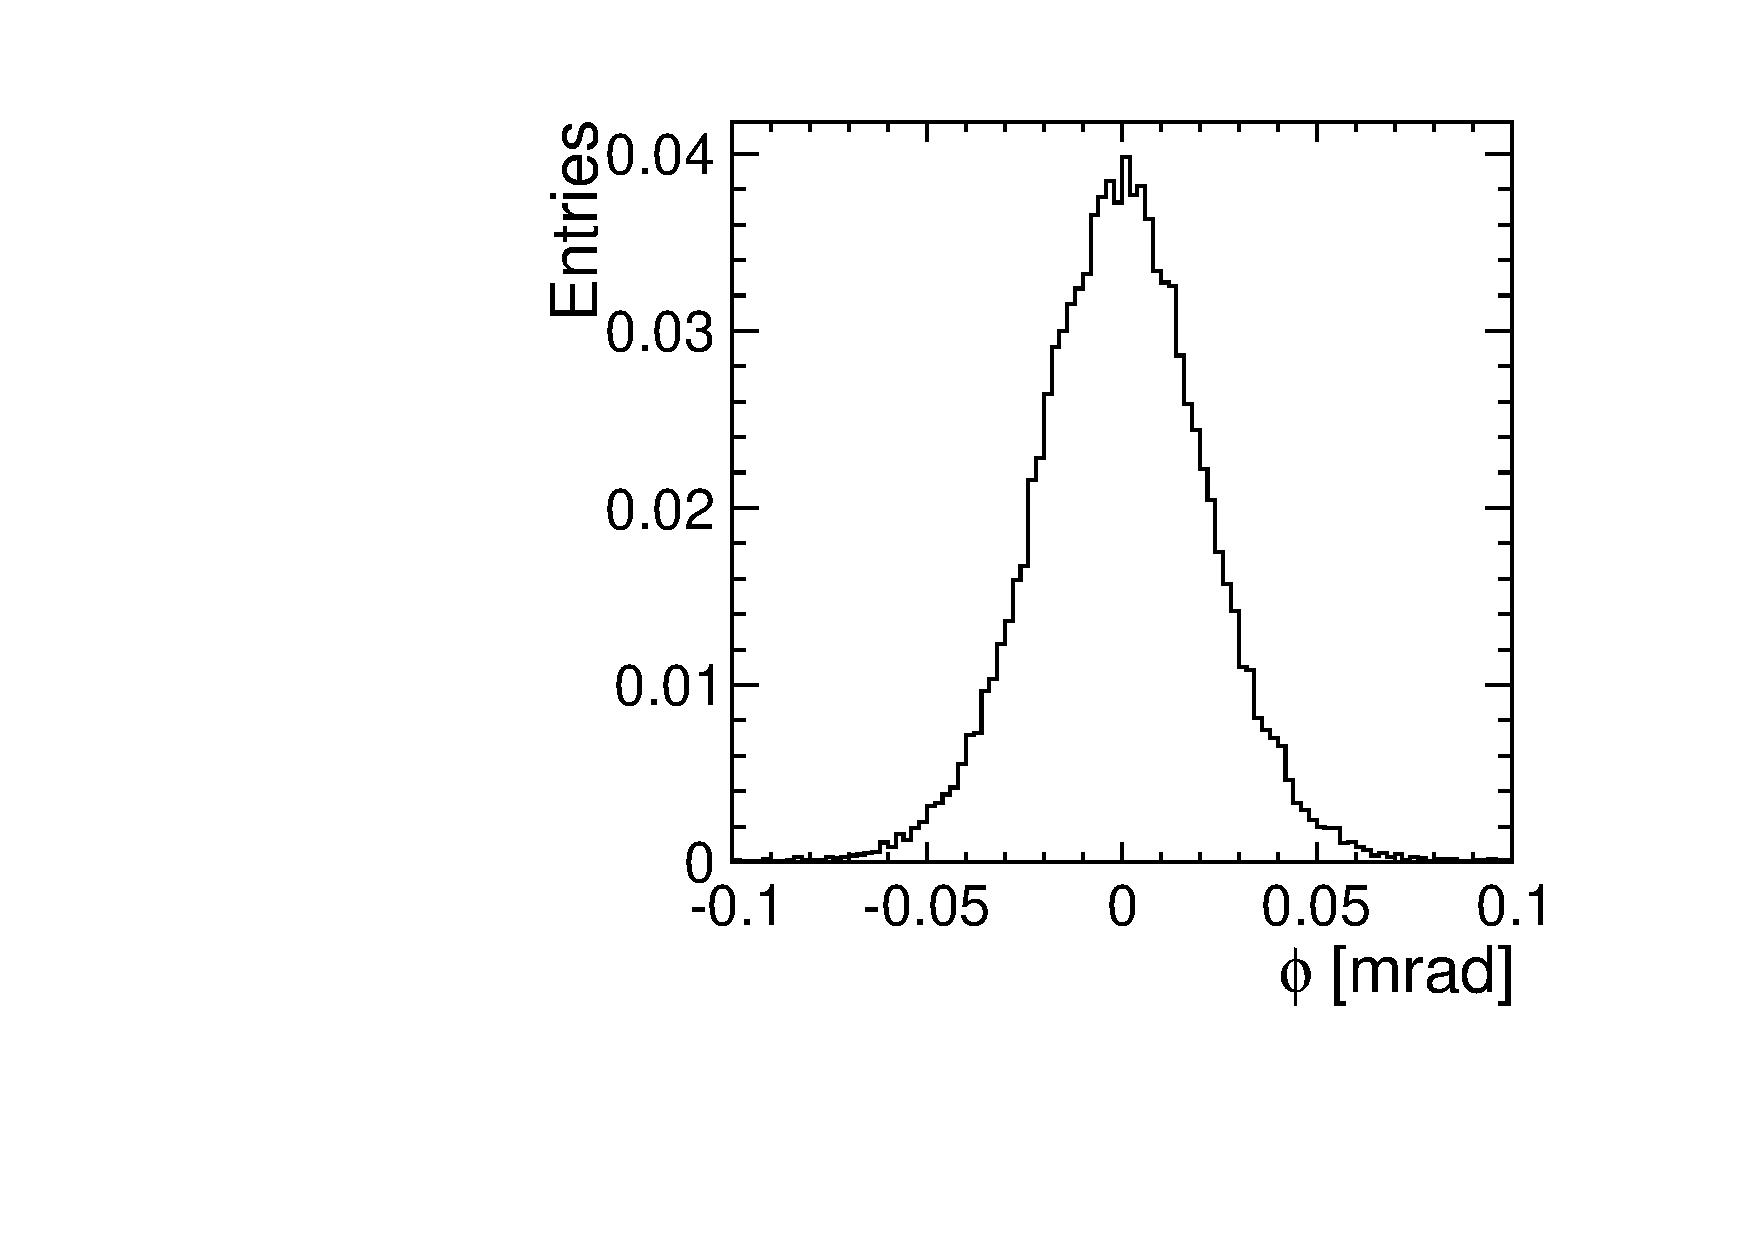
\includegraphics[width=\textwidth]{./figures/Telescope/MC_trackAnglePhi_planes_302_100.pdf}
    \caption{}
  \end{subfigure}\hfill
  \begin{subfigure}[b]{0.45\textwidth}
    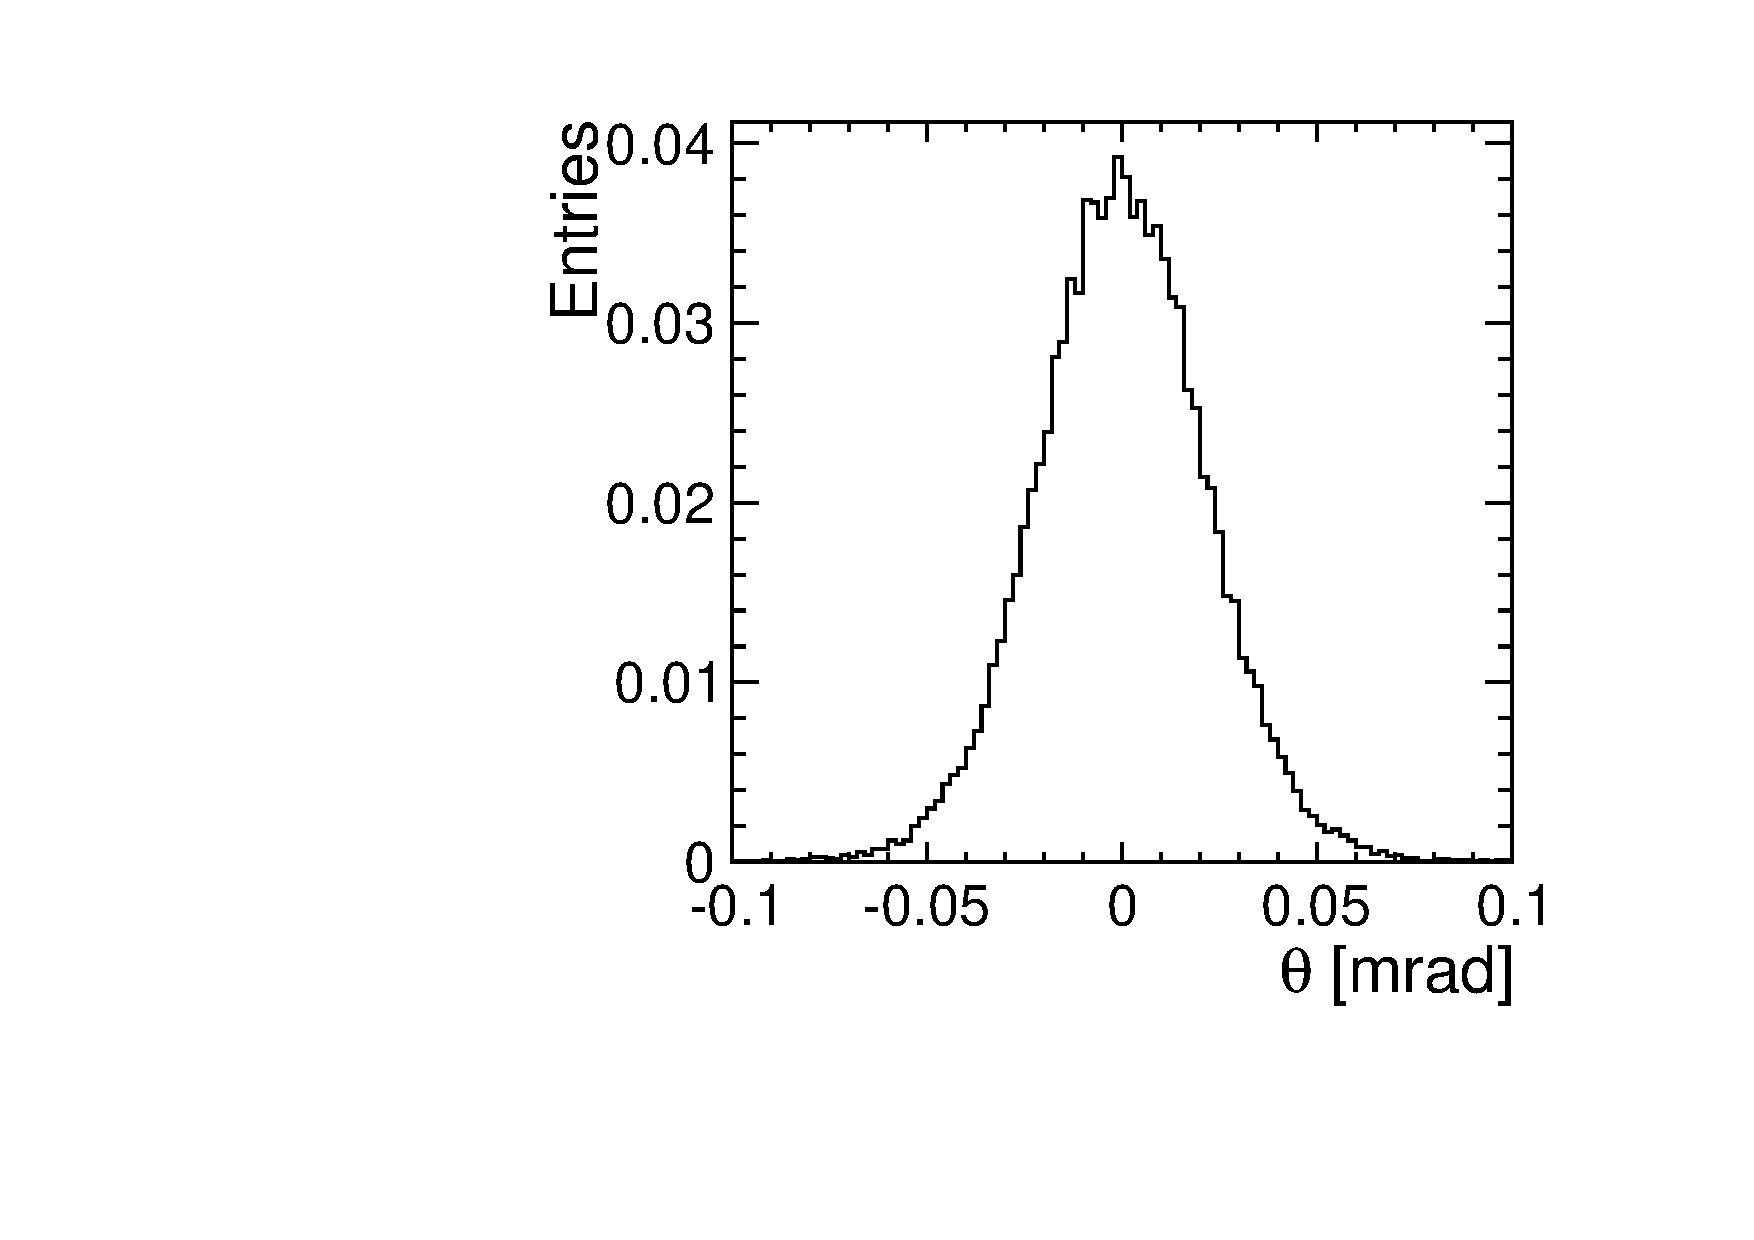
\includegraphics[width=\textwidth]{./figures/Telescope/MC_trackAngleTheta_planes_302_100.pdf}
    \caption{}
  \end{subfigure}
  \caption{Beam angular distribution in \textsc{Geant4} simulations
(comparing the global positions on the second telescope plane and on
the DUT).}
  \label{fig:MCbeamAngleDistr}
\end{figure}
